\newpage
\chapter[Finite Element Formulation]{Governing Equations and Finite Element Formulation}\label{chap:governing-equations}

The preceding chapters used finite element matrices such as $\m{K}$, $\m{M}$ and
$\m{f}$ as already existing objects. That is appropriate when the subject is a
boundary condition, a constraint, contact or a kinematic coupling. At some point,
however, the more fundamental question has to be answered:

\begin{center}
\textit{Where do the element matrices actually come from?}
\end{center}

This chapter follows the complete chain from continuum mechanics to the loops
executed by a finite element program:

\begin{center}
\textbf{engineering behaviour}
$\longleftrightarrow$
\textbf{continuum equations}
$\longleftrightarrow$
\textbf{weak form}
$\longleftrightarrow$
\textbf{discrete element}
$\longleftrightarrow$
\textbf{implementation}.
\end{center}

The objective is not to reproduce an element catalogue. Chapter~11 is intended
for that purpose. Instead, the objective here is to explain enough of the
mathematics and implementation that an analyst can understand, modify and, when
necessary, derive an element formulation of his or her own.

\begin{figure}[ht]
    \centering
    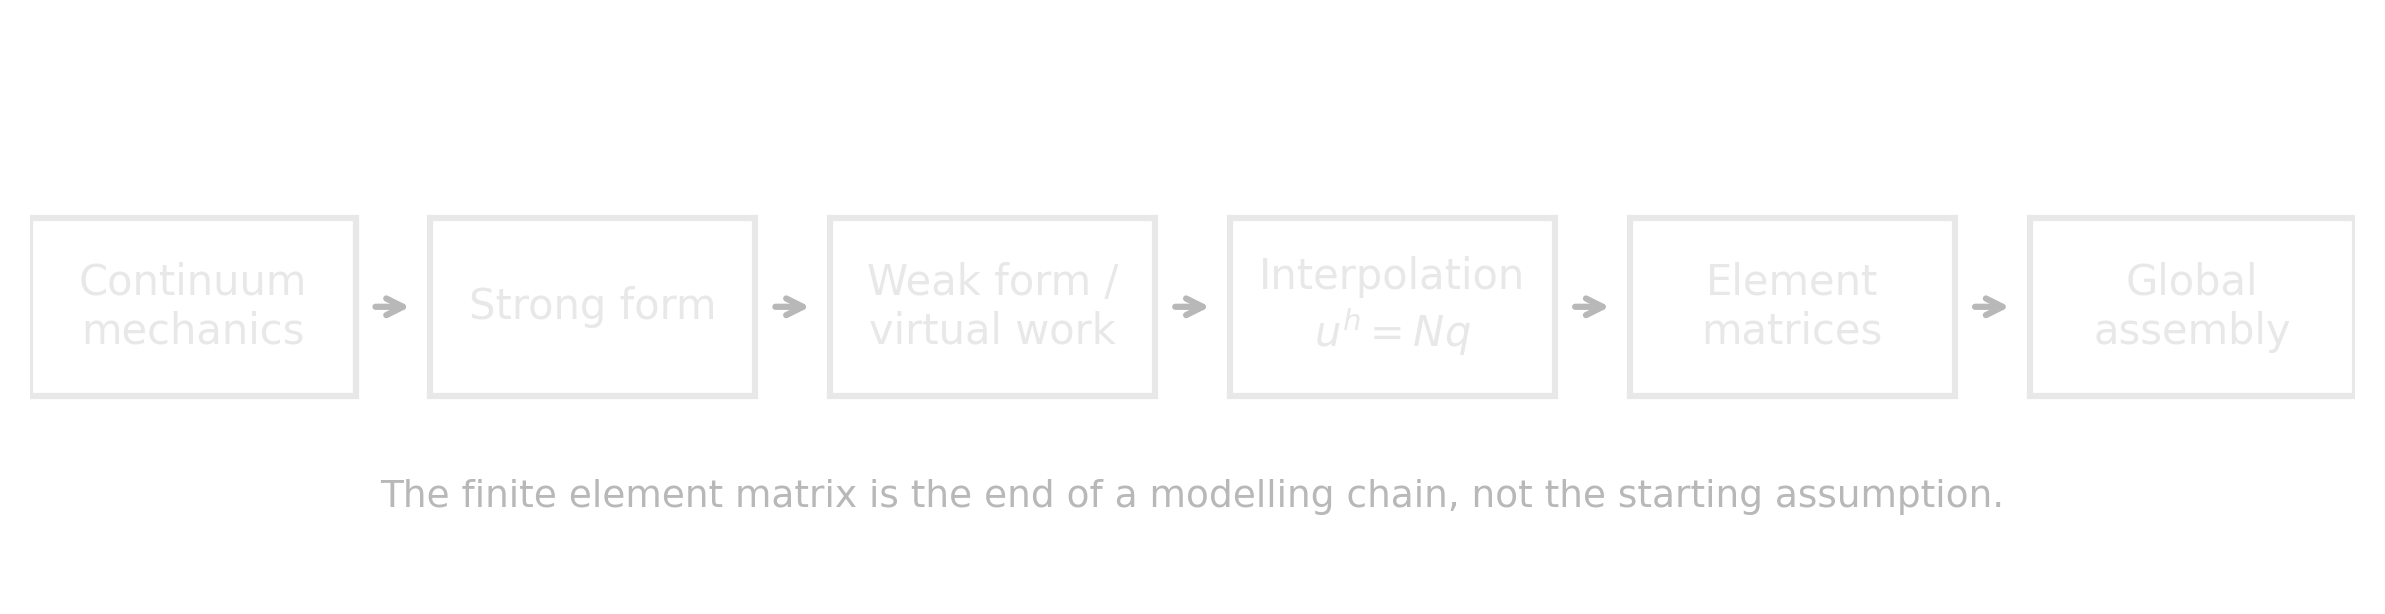
\includegraphics[width=0.95\textwidth]{img/fe_continuum_to_discrete.png}
    \caption{The finite element matrix is the end of a modelling chain. The
    governing continuum equations are first converted to a variational form,
    approximated by finite-dimensional interpolation and only then assembled
    into algebraic matrices.}
    \label{fig:fe-continuum-to-discrete}
\end{figure}

\begin{bbox}
\textbf{Python examples in this chapter.}

As in Chapters~1--5, the code is intentionally transparent. \texttt{numpy} is
used for arrays, indexing, elementary arithmetic and matrix products. No
\texttt{numpy.linalg}, sparse solver, eigensolver or other high-level numerical
submodule is used. Small dense systems, $3\times3$ determinants and inverses are
implemented explicitly so that the transition from the equations to actual
loops remains visible.

The examples are educational element kernels, not production finite element
software. A production code additionally needs sparse storage, robust geometry
handling, material state management, parallel assembly, error control and many
other layers that are deliberately kept outside the examples here.
\end{bbox}

\section{The Continuum Problem}

A finite element is a discrete approximation to a continuum problem. For a
small-strain elastic solid, the essential fields are

\begin{equation}
    \m{u}(\m{x}),\qquad
    \M{\varepsilon}(\m{x}),\qquad
    \M{\sigma}(\m{x}),
\end{equation}

representing displacement, strain and stress. They are linked by three distinct
pieces of physics:

\begin{enumerate}
    \item \textbf{kinematics}: displacement determines strain,
    \item \textbf{constitutive behaviour}: strain determines stress,
    \item \textbf{equilibrium}: stress must balance the applied loading.
\end{enumerate}

It is useful to keep these three roles conceptually separate. A poor finite
element may use the correct material law and satisfy the algebraic equilibrium
equations while still behaving badly because its discrete kinematics are too
restrictive. Shear locking, volumetric locking and many other element pathologies
are examples of precisely this problem.

\subsection{Small-Strain Kinematics}

For a three-dimensional displacement field

\begin{equation}
    \m{u}=\begin{bmatrix}u&v&w\end{bmatrix}^T,
\end{equation}

the displacement gradient is

\begin{equation}
    \nabla\m{u}
    =
    \begin{bmatrix}
        u_{,x} & u_{,y} & u_{,z}\\
        v_{,x} & v_{,y} & v_{,z}\\
        w_{,x} & w_{,y} & w_{,z}
    \end{bmatrix}.
\end{equation}

Its symmetric part gives the infinitesimal strain tensor,

\begin{equation}\label{eq:small-strain-tensor}
    \boxed{
    \M{\varepsilon}
    =\operatorname{sym}(\nabla\m{u})
    =\frac{1}{2}
    \left(
        \nabla\m{u}+(\nabla\m{u})^T
    \right)}.
\end{equation}

Using engineering shear strains, the strain vector is commonly stored as

\begin{equation}\label{eq:engineering-strain-vector}
    \M{\varepsilon}_v
    =
    \begin{bmatrix}
        \varepsilon_{xx}&
        \varepsilon_{yy}&
        \varepsilon_{zz}&
        \gamma_{xy}&
        \gamma_{yz}&
        \gamma_{zx}
    \end{bmatrix}^T.
\end{equation}

The factor of two hidden in the engineering shear components is important. A
constitutive matrix written for tensorial shear strains cannot be mixed with a
$\M{\varepsilon}_v$ vector containing engineering shear strains.

\subsection{Finite Kinematics in Brief}

Small strain does not mean small displacement, and a general nonlinear element
cannot use Equation~\eqref{eq:small-strain-tensor} after large rotations without
additional care. In the reference configuration $\m{X}$, the deformation map
$\m{x}=\M{\varphi}(\m{X})$ defines the deformation gradient

\begin{equation}
    \boxed{
    \m{F}=\frac{\partial\m{x}}{\partial\m{X}}
    =\m{I}+\frac{\partial\m{u}}{\partial\m{X}}
    }.
\end{equation}

A common finite-strain measure is the Green--Lagrange strain

\begin{equation}
    \m{E}
    =\frac{1}{2}(\m{F}^T\m{F}-\m{I}).
\end{equation}

The present chapter derives the linear small-strain element first because the
entire discrete structure is easiest to see there. In a nonlinear formulation
the same ideas reappear in residual and tangent form: the kinematics,
constitutive response and geometry are evaluated at the current state and the
element tangent is rebuilt during the iteration.

\subsection{Constitutive Relation}

For linear elasticity the stress and strain vectors are related by

\begin{equation}\label{eq:linear-constitutive}
    \boxed{
    \M{\sigma}_v=\m{D}\M{\varepsilon}_v
    }.
\end{equation}

The matrix $\m{D}$ contains the constitutive law. For an isotropic three-
dimensional solid it depends only on Young's modulus $E$ and Poisson's ratio
$\nu$. For a composite, anisotropic solid, plastic material, hyperelastic
material or a user-defined law, this constitutive mapping is different, but the
surrounding finite element machinery remains conceptually the same.

\section[Reference Matrices]{Reference: Generalised Kinematic and Constitutive Matrices}

The following tables provide a compact engineering reference. They collect the kinematic quantities and the common isotropic
constitutive matrices used in several standard problem reductions. Some rows,
such as the beam and plate rows, contain \textit{generalised section stiffness}
rather than a three-dimensional material matrix. That distinction is noted
because the same matrix notation is often used for both in engineering texts.

\begin{notebooknote}[Reference material is allowed to interrupt the narrative]
This book has two jobs: to explain a formulation when it is being studied, and
to make the useful result easy to find months or years later.  Compact lookup
tables, derivations kept for reference, and apparently specialised side results
are useful when they save having to derive the same thing again.
They are part of the engineering notebook rather than editorial clutter.
\end{notebooknote}

\begin{table}[ht]
    \centering
    \renewcommand{\arraystretch}{1.25}
    \scalebox{0.83}{
    \begin{tabular}{||c c c c||}
        \hline
        \hline
        Problem & \begin{tabular}{c}Displacement\\components\\ \end{tabular} &
        Strain vector $ \M{\epsilon}^T $ & Stress vector $ \M{\tau}^T $ \\
        \hline
        Bar & $u$ & $ \left[ \epsilon_{xx} \right] $ & $ \left[ \sigma_{xx} \right] $ \\
        Beam & $w$ & $ \left[ \kappa_{xx} \right] $ & $ \left[ m_{xx} \right] $ \\
        Plane stress & $u,v$ & $ \left[ \epsilon_{xx}, \epsilon_{yy}, \gamma_{xy} \right] $
                     & $ \left[ \sigma_{xx}, \sigma_{yy}, \tau_{xy} \right] $ \\
        Plane strain & $u,v$ & $ \left[ \epsilon_{xx}, \epsilon_{yy}, \gamma_{xy} \right] $
                     & $ \left[ \sigma_{xx}, \sigma_{yy}, \tau_{xy} \right] $ \\
        Axisymmetric & $u,v$
                     & $ \left[ \epsilon_{xx}, \epsilon_{yy}, \gamma_{xy}, \epsilon_{zz} \right] $
                     & $ \left[ \sigma_{xx}, \sigma_{yy}, \tau_{xy}, \sigma_{zz} \right] $ \\
        3D & $u,v,w$
           & $ \left[ \epsilon_{xx}, \epsilon_{yy}, \epsilon_{zz},
           \gamma_{xy}, \gamma_{yz}, \gamma_{zx} \right] $
                     & $ \left[ \sigma_{xx}, \sigma_{yy}, \sigma_{zz},
                     \tau_{xy}, \tau_{yz}, \tau_{zx} \right] $ \\
        Plate bending & $w$ & $ \left[ \kappa_{xx}, \kappa_{yy}, \kappa_{xy} \right] $ &
                             $ \left[ m_{xx}, m_{yy}, m_{xy} \right] $ \\
        \hline
        \hline
        \multicolumn{4}{l}{
            Notation:
            $ \epsilon_{xx} = \frac{\partial u}{\partial x} $,
            $ \epsilon_{yy} = \frac{\partial v}{\partial y} $,
            $ \gamma_{xy} = \frac{\partial u}{\partial y} + \frac{\partial v}{\partial x} $,
            $ \dots $,
            $ \kappa_{xx} = \frac{\partial^2 w}{\partial x^2} $,
            $ \kappa_{yy} = \frac{\partial^2 w}{\partial y^2} $,
            $ \kappa_{xy} = \frac{\partial^2 w}{\partial x \partial y} $.
        } \\
    \end{tabular}}
    \caption{Corresponding kinematic and static variables in various problems.}
    \label{tab:generalized-kinematic-static-vars}
\end{table}

\begin{table}[ht]
    \centering
    \renewcommand{\arraystretch}{2.00}
    \scalebox{0.73}{
    \begin{tabular}{||c c||}
        \hline
        \hline
        Problem & Material or generalised constitutive matrix $ D $ \\
        \hline
        Bar & $ E $ \\
        Beam & $ E I $ \\
        Plane stress & \begin{math}
            \frac{E}{1 - \nu^2}
            \begin{bmatrix}
                1 & \nu & 0 \\
                \nu & 1 & 0 \\
                0 & 0 & \frac{1 - \nu}{2}
            \end{bmatrix}
        \end{math} \\
        Plane strain & \begin{math}
            \frac{E\left(1 - \nu\right)}{\left(1 + \nu\right)\left(1 - 2\nu\right)}
            \begin{bmatrix}
                1 & \frac{\nu}{1 - \nu} & 0 \\
                \frac{\nu}{1 - \nu} & 1 & 0 \\
                0 & 0 & \frac{1 - 2 \nu}{2 \left(1 - \nu\right)}
            \end{bmatrix}
        \end{math} \\
        Axisymmetric & \begin{math}
            \frac{E\left(1 - \nu\right)}{\left(1 + \nu\right)\left(1 - 2\nu\right)}
            \begin{bmatrix}
                1 & \frac{\nu}{1 - \nu} & 0 & \frac{\nu}{1 - \nu} \\
                \frac{\nu}{1 - \nu} & 1 & 0 & \frac{\nu}{1 - \nu} \\
                0 & 0 & \frac{1 - 2 \nu}{2 \left(1 - \nu\right)} & 0 \\
                \frac{\nu}{1-\nu} & \frac{\nu}{1-\nu} & 0 & 1
            \end{bmatrix}
        \end{math} \\
        3D & \begin{math}
            \frac{E\left(1 - \nu\right)}{\left(1 + \nu\right)\left(1 - 2\nu\right)}
            \begin{bmatrix}
                1 & \frac{\nu}{1 - \nu} & \frac{\nu}{1 - \nu} & 0 & 0 & 0 \\
                \frac{\nu}{1 - \nu} & 1 & \frac{\nu}{1 - \nu} & 0 & 0 & 0 \\
                \frac{\nu}{1 - \nu} & \frac{\nu}{1 - \nu} & 1 & 0 & 0 & 0 \\
                0 & 0 & 0 & \frac{1 - 2 \nu}{2 \left(1 - \nu \right)} & 0 & 0 \\
                0 & 0 & 0 & 0 & \frac{1 - 2 \nu}{2 \left(1 - \nu \right)} & 0 \\
                0 & 0 & 0 & 0 & 0 & \frac{1 - 2 \nu}{2 \left(1 - \nu \right)}
            \end{bmatrix}
        \end{math} \\
        Plate bending & \begin{math}
            \frac{E h^3}{12 \left(1 - \nu^2 \right)}
            \begin{bmatrix}
                1 & \nu & 0 \\
                \nu & 1 & 0 \\
                0 & 0 & \frac{1 - \nu}{2}
            \end{bmatrix}
        \end{math} \\
        \hline
        \hline
        \multicolumn{2}{l}{
            Notation:
            $ E = $ Young's modulus, $ \nu = $ Poisson's ratio,
            $ h = $ thickness of plate, $ I = $ second moment of area
        } \\
    \end{tabular}}
    \caption{Common isotropic material and generalised section matrices.}
    \label{tab:common-material-matrices}
\end{table}

\section{Strong Form of Equilibrium}

For a static continuum occupying $\Omega$ with boundary $\Gamma$, local
balance of linear momentum requires

\begin{equation}\label{eq:strong-equilibrium}
    \boxed{
    \nabla\!\cdot\M{\sigma}+\m{b}=\m{0}
    \qquad\text{in }\Omega
    },
\end{equation}

where $\m{b}$ is the body force per unit volume. In dynamics,

\begin{equation}
    \rho\ddot{\m{u}}
    =\nabla\!\cdot\M{\sigma}+\m{b}.
\end{equation}

The boundary is divided into a displacement part $\Gamma_u$ and a traction part
$\Gamma_t$,

\begin{align}
    \m{u}&=\bar{\m{u}}
        &&\text{on }\Gamma_u,\\
    \M{\sigma}\m{n}&=\bar{\m{t}}
        &&\text{on }\Gamma_t.
\end{align}

These are exactly the Dirichlet and Neumann conditions introduced in
Chapter~2. In the strong form they look symmetric on paper, but they enter the
finite element formulation differently: the displacement condition restricts
the admissible approximation space, while the traction appears naturally in
the weak-form load vector.

\begin{bbox}
\textbf{Engineering note -- Why not discretise the strong form directly?}

Equation~\eqref{eq:strong-equilibrium} contains spatial derivatives of stress,
and therefore higher derivatives of displacement. Requiring an approximate
finite element displacement to satisfy this differential equation pointwise is
unnecessarily restrictive for many useful element interpolations. The weak form
moves one derivative from the trial displacement to a virtual/test field and
thereby lowers the continuity required between elements.
\end{bbox}

\section{Principle of Virtual Work}

Let $\delta\m{u}$ be an arbitrary virtual displacement that satisfies the
homogeneous form of the essential boundary conditions,

\begin{equation}
    \delta\m{u}=\m{0}\qquad\text{on }\Gamma_u.
\end{equation}

Multiplying Equation~\eqref{eq:strong-equilibrium} by $\delta\m{u}$, integrating
over the domain and applying integration by parts gives

\begin{equation}\label{eq:virtual-work-continuum}
    \boxed{
    \int_{\Omega}
    \delta\M{\varepsilon}^T\M{\sigma}\,d\Omega
    =
    \int_{\Omega}\delta\m{u}^T\m{b}\,d\Omega
    +
    \int_{\Gamma_t}\delta\m{u}^T\bar{\m{t}}\,d\Gamma
    }.
\end{equation}

The left side is the virtual internal work and the right side the virtual
external work. This equation is often the most convenient starting point for a
new displacement-based element because the constitutive law, interpolation and
external loading all enter transparently.

\section{The Deformation-Energy Route}

The same linear elastic element matrix can be obtained from strain energy. The
stored deformation energy is

\begin{equation}
    U
    =\frac{1}{2}
    \int_{\Omega}
    \M{\varepsilon}^T\m{D}\M{\varepsilon}\,d\Omega.
\end{equation}

For conservative external loads with potential $W_{\mathrm{ext}}$, define the
total potential energy

\begin{equation}
    \Pi=U-W_{\mathrm{ext}}.
\end{equation}

Equilibrium follows from stationarity,

\begin{equation}
    \delta\Pi=0.
\end{equation}

The virtual-work and strain-energy routes are therefore not competing element
theories. For a conservative linear elastic problem they are two views of the
same equilibrium statement.

\begin{figure}[ht]
    \centering
    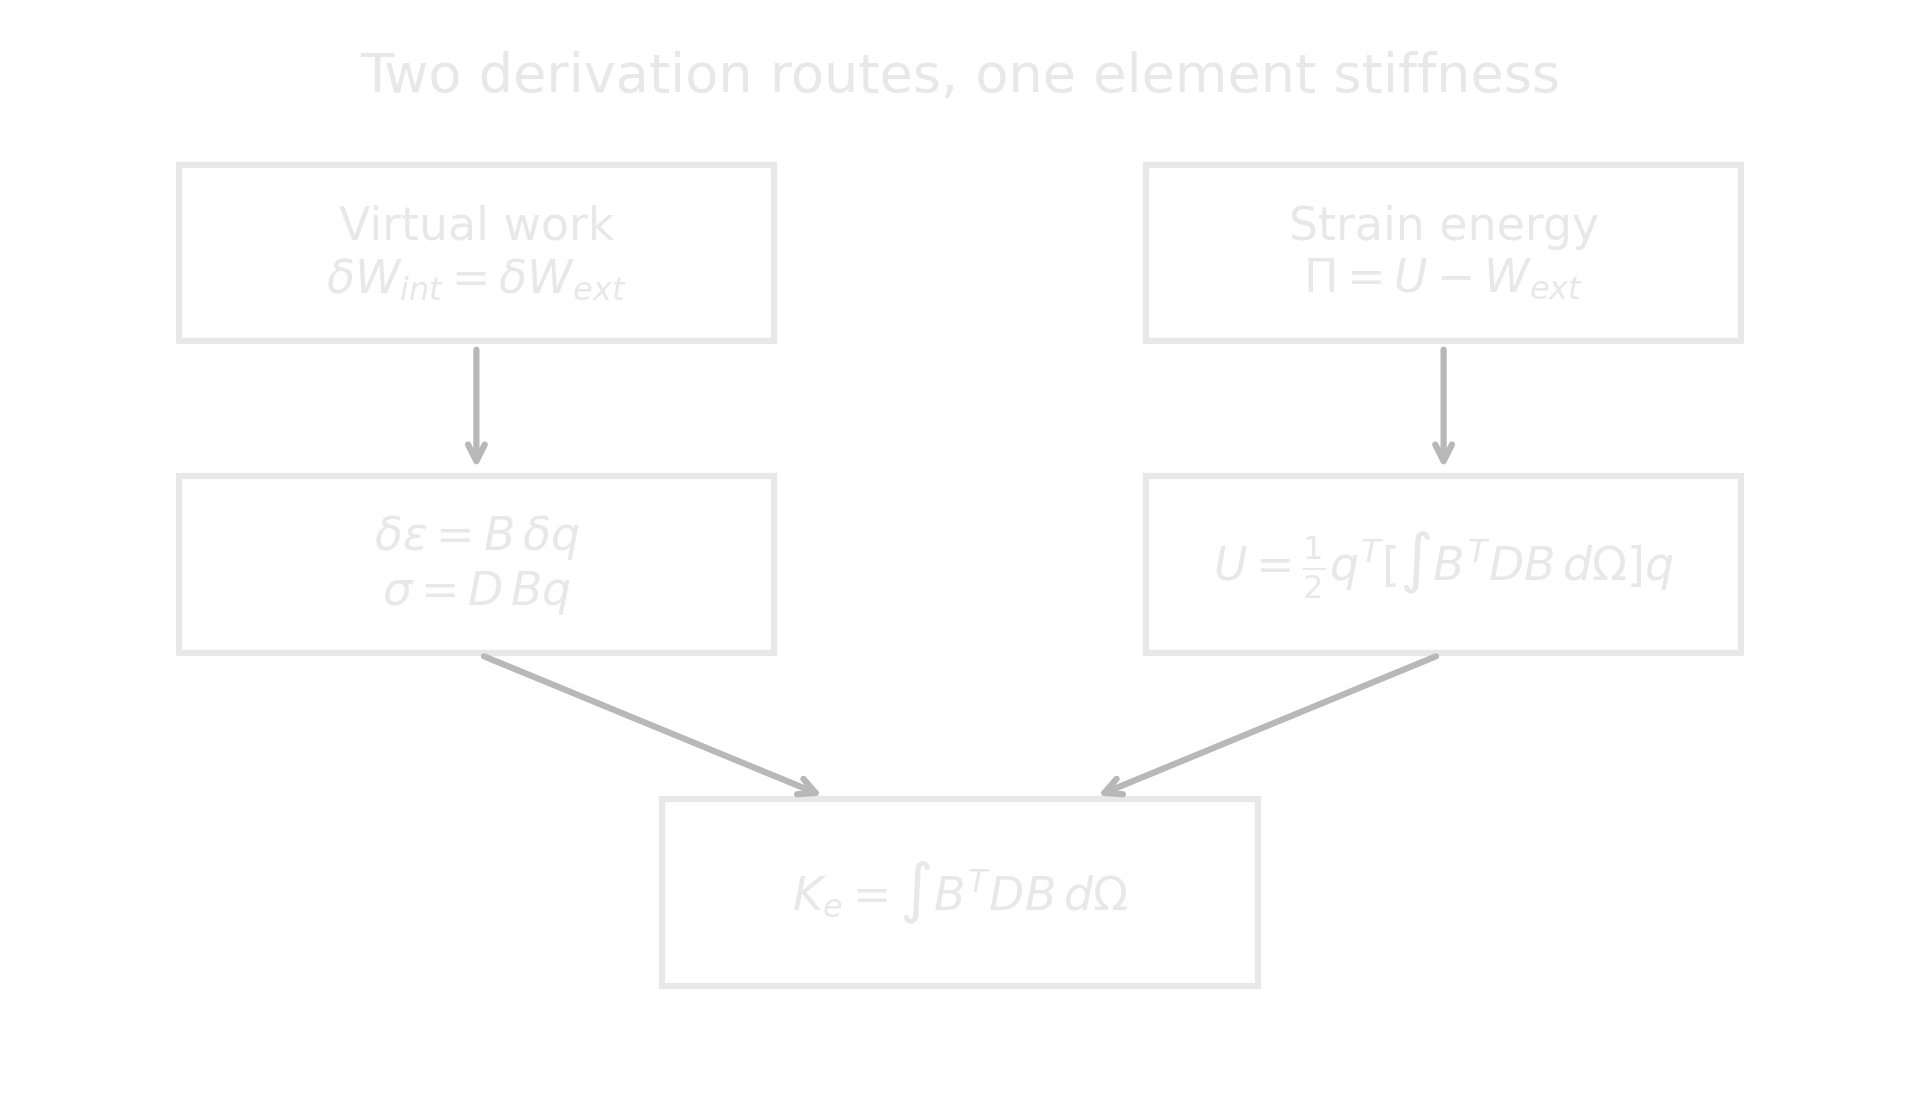
\includegraphics[width=0.77\textwidth]{img/fe_virtual_work_energy_routes.png}
    \caption{Two common derivation routes for a linear elastic element. Virtual
    work starts from equilibrium; the deformation-energy route starts from
    stored energy. After finite-dimensional interpolation both lead to the same
    element stiffness.}
    \label{fig:fe-two-derivation-routes}
\end{figure}

\section{Finite-Dimensional Approximation}

The finite element approximation replaces the continuous displacement field by
a finite set of nodal or generalised coordinates $\m{q}_e$,

\begin{equation}\label{eq:fe-interpolation}
    \boxed{
    \m{u}^h(\m{x})=\m{N}(\m{x})\m{q}_e
    }.
\end{equation}

The interpolation matrix $\m{N}$ contains the shape functions. For an ordinary
nodal displacement element, a shape function should normally satisfy the
Kronecker-delta property

\begin{equation}
    N_i(\m{x}_j)=\delta_{ij},
\end{equation}

so that the interpolation reproduces the nodal coordinates exactly.

Three properties are particularly important when designing an approximation
space:

\begin{itemize}
    \item \textbf{partition of unity}: $\sum_iN_i=1$, so rigid translation is
          reproduced;
    \item \textbf{completeness}: the interpolation can reproduce the polynomial
          fields required for the intended convergence order;
    \item \textbf{compatibility}: neighbouring elements satisfy the continuity
          requirements of the weak form.
\end{itemize}

For small strain, substituting Equation~\eqref{eq:fe-interpolation} into the
kinematic relation gives

\begin{equation}\label{eq:Bq}
    \boxed{
    \M{\varepsilon}=\m{B}\m{q}_e
    },
\end{equation}

where $\m{B}$ is the strain-displacement matrix assembled from derivatives of
$\m{N}$.

\subsection{From Virtual Work to the Element Matrix}

Substitute

\begin{equation}
    \delta\m{u}=\m{N}\delta\m{q}_e,
    \qquad
    \delta\M{\varepsilon}=\m{B}\delta\m{q}_e,
    \qquad
    \M{\sigma}=\m{D}\m{B}\m{q}_e
\end{equation}

into Equation~\eqref{eq:virtual-work-continuum}. Because
$\delta\m{q}_e$ is arbitrary,

\begin{equation}\label{eq:element-stiffness}
    \boxed{
    \m{K}_e
    =
    \int_{\Omega_e}
    \m{B}^T\m{D}\m{B}\,d\Omega
    },
\end{equation}

and

\begin{equation}\label{eq:element-load}
    \boxed{
    \m{f}_e
    =
    \int_{\Omega_e}\m{N}^T\m{b}\,d\Omega
    +
    \int_{\Gamma_t^e}\m{N}^T\bar{\m{t}}\,d\Gamma
    }.
\end{equation}

The energy route produces exactly the same result because

\begin{equation}
    U_e
    =\frac{1}{2}\m{q}_e^T\m{K}_e\m{q}_e.
\end{equation}

The internal nodal force is therefore

\begin{equation}
    \m{f}_{\mathrm{int},e}
    =\frac{\partial U_e}{\partial\m{q}_e}
    =\m{K}_e\m{q}_e
\end{equation}

for the linear elastic case.

\subsection{Mass Matrix}

The kinetic energy of the element is

\begin{equation}
    T_e
    =\frac{1}{2}
    \int_{\Omega_e}
    \rho\dot{\m{u}}^T\dot{\m{u}}\,d\Omega.
\end{equation}

Using $\dot{\m{u}}=\m{N}\dot{\m{q}}_e$ gives the consistent mass matrix

\begin{equation}\label{eq:consistent-mass}
    \boxed{
    \m{M}_e
    =\int_{\Omega_e}
    \rho\m{N}^T\m{N}\,d\Omega
    }.
\end{equation}

A lumped mass matrix replaces this distributed coupling by diagonal nodal masses.
Lumping may be desirable in explicit dynamics, but it is a numerical modelling
choice rather than a consequence of the continuum kinetic energy itself.

\section{Isoparametric Mapping and the Jacobian}

Most practical continuum elements are formulated in a simple natural-coordinate
domain $\M{\xi}=(\xi,\eta,\zeta)$ and mapped to the physical element geometry.
For an isoparametric element, the same scalar shape functions are used for
geometry and displacement interpolation,

\begin{align}
    \m{x}(\M{\xi}) &= \sum_iN_i(\M{\xi})\m{x}_i,\\
    \m{u}^h(\M{\xi}) &= \sum_iN_i(\M{\xi})\m{u}_i.
\end{align}

The Jacobian matrix

\begin{equation}\label{eq:isoparametric-jacobian}
    \m{J}
    =\frac{\partial\m{x}}{\partial\M{\xi}}
\end{equation}

maps natural-coordinate derivatives to physical derivatives. With the row-vector
convention used in the code examples,

\begin{equation}
    \begin{bmatrix}
        N_{,x}&N_{,y}&N_{,z}
    \end{bmatrix}
    =
    \begin{bmatrix}
        N_{,\xi}&N_{,\eta}&N_{,\zeta}
    \end{bmatrix}
    \m{J}^{-1}.
\end{equation}

The volume differential transforms as

\begin{equation}
    d\Omega=\det(\m{J})\,d\xi\,d\eta\,d\zeta.
\end{equation}

A negative or vanishing determinant is therefore not merely a geometric warning.
It directly breaks the mapping used to calculate physical gradients and
integration weights.

\section{Numerical Integration}

After mapping to the natural element, Equation~\eqref{eq:element-stiffness} is
usually evaluated by quadrature,

\begin{equation}
    \m{K}_e
    \approx
    \sum_{g=1}^{n_g}
    \m{B}_g^T\m{D}_g\m{B}_g
    \det(\m{J}_g)w_g.
\end{equation}

Thus the integral sign becomes a loop over integration points. At each point the
program must

\begin{enumerate}
    \item evaluate shape functions and natural derivatives,
    \item construct $\m{J}$,
    \item transform derivatives to physical coordinates,
    \item build $\m{B}$,
    \item evaluate the constitutive matrix or material algorithm,
    \item accumulate the weighted contribution.
\end{enumerate}

The Element Atlas contains the longer quadrature reference. Here the important
point is conceptual: integration order is part of the element formulation. Too
few points can create zero-energy modes; too many points do not necessarily
improve a locking-prone interpolation and may actually enforce an undesirable
constraint more strongly.

\section{A Minimal Element Kernel in Python}

Before developing more sophisticated elements, it is useful to make the matrix
operations explicit. The following utilities are used by the later HEX8
examples. The $3\times3$ inverse is written directly from cofactors rather than
calling a library routine.

\begin{python}
import math
import numpy as np


def inverse_3x3(A):
    a, b, c = A[0]
    d, e, f = A[1]
    g, h, i = A[2]

    adj = np.array([
        [e*i - f*h, c*h - b*i, b*f - c*e],
        [f*g - d*i, a*i - c*g, c*d - a*f],
        [d*h - e*g, b*g - a*h, a*e - b*d],
    ], dtype=float)

    det = a*adj[0, 0] + b*adj[1, 0] + c*adj[2, 0]
    if abs(det) < 1.0e-14:
        raise ValueError("singular 3x3 matrix")

    return adj / det, det


def solve_dense(A, B):
    """Gaussian elimination with partial pivoting; B may have many columns."""
    A = np.array(A, dtype=float, copy=True)
    B = np.array(B, dtype=float, copy=True)
    if B.ndim == 1:
        B = B.reshape((-1, 1))

    n = A.shape[0]
    for k in range(n):
        pivot = k
        for i in range(k + 1, n):
            if abs(A[i, k]) > abs(A[pivot, k]):
                pivot = i
        if abs(A[pivot, k]) < 1.0e-14:
            raise ValueError("singular matrix")

        if pivot != k:
            A[[k, pivot]] = A[[pivot, k]]
            B[[k, pivot]] = B[[pivot, k]]

        for i in range(k + 1, n):
            factor = A[i, k] / A[k, k]
            A[i, k:] -= factor * A[k, k:]
            B[i, :] -= factor * B[k, :]

    X = np.zeros_like(B)
    for col in range(B.shape[1]):
        for i in range(n - 1, -1, -1):
            rhs = B[i, col]
            for j in range(i + 1, n):
                rhs -= A[i, j] * X[j, col]
            X[i, col] = rhs / A[i, i]

    return X[:, 0] if X.shape[1] == 1 else X
\end{python}

The function is not meant to compete with a numerical linear algebra library.
Its purpose is to expose that static condensation or a small local coordinate
transformation eventually becomes pivot selection, elimination and back
substitution in a program.

\section{Global Assembly}

Let $\m{L}_e$ map the element DOFs into the global vector,

\begin{equation}
    \m{q}_e=\m{L}_e\m{u}.
\end{equation}

The global stiffness is commonly written compactly as

\begin{equation}
    \boxed{
    \m{K}=\sum_e\m{L}_e^T\m{K}_e\m{L}_e
    }.
\end{equation}

In code this is an index-scatter operation. The matrix $\m{L}_e$ is almost never
formed explicitly:

\begin{python}
def assemble_element_matrix(K, Ke, dofs):
    for a, I in enumerate(dofs):
        for b, J in enumerate(dofs):
            K[I, J] += Ke[a, b]


def assemble_element_vector(f, fe, dofs):
    for a, I in enumerate(dofs):
        f[I] += fe[a]
\end{python}

The mathematical summation symbol has therefore become two nested loops and a
DOF map. This transition from local mathematical notation to indexing and
accumulation is one of the most fundamental implementation ideas in finite
element programming.


\section{Choosing the Approximation Space}\label{sec:fe-approximation-space}

The finite element method does not require Lagrange polynomials.  What the
method requires is a finite-dimensional trial space that is compatible with the
variational problem and rich enough to represent the deformation states that
matter.  The familiar nodal interpolation

\begin{equation}
    \m{u}^{h}(\m{x})=\sum_a N_a(\m{x})\m{q}_a
\end{equation}

therefore hides one of the most important design decisions in an element: the
choice of the functions $N_a$ and of the generalized coordinates that multiply
them.

Lagrange polynomials are popular because they combine several useful properties:

\begin{itemize}
    \item the Kronecker property $N_i(\m{x}_j)=\delta_{ij}$ gives the
          coefficients a direct nodal interpretation,
    \item partition of unity reproduces rigid translations,
    \item polynomial completeness makes constant-strain and higher-order patch
          tests straightforward,
    \item local support preserves sparse FE assembly,
    \item derivatives and Gauss integration are inexpensive.
\end{itemize}

None of these properties is unique to Lagrange polynomials.  Other useful
families include

\begin{center}
\begin{tabular}{>{\raggedright\arraybackslash}p{0.20\textwidth}>{\raggedright\arraybackslash}p{0.30\textwidth}>{\raggedright\arraybackslash}p{0.30\textwidth}}
\hline
\textbf{Basis family} & \textbf{Why it is attractive} & \textbf{Typical use}\\
\hline
Lagrange polynomial & direct nodal values, simple $C^0$ assembly & standard solids and thermal elements\\
Hermite polynomial & values and slopes are interpolation data & beams and $C^1$ problems\\
Hierarchical polynomial & additional modes can be added without replacing the lower-order basis & $p$- and $hp$-refinement\\
Trigonometric / Fourier & represents periodic and oscillatory fields efficiently & cyclic structures, spectral approximations\\
Exponential / wave & follows the local solution of a propagation problem & dynamic stiffness and wave elements\\
Spline/NURBS & high continuity and accurate geometric representation & isogeometric analysis\\
Problem-specific enrichment & adds a known local deformation, singularity or discontinuity & incompatible modes, XFEM, partition-of-unity methods\\
\hline
\end{tabular}
\end{center}

A non-polynomial basis is therefore not an exotic departure from FEM.  It is
simply a different finite-dimensional approximation space.  The questions that
must be asked are more fundamental:

\begin{enumerate}
    \item \textbf{Completeness.} Does the space reproduce rigid-body motion and
          the low-order strain states required for convergence?
    \item \textbf{Compatibility.} Does the assembled field have the continuity
          required by the weak form?
    \item \textbf{Stability.} Does the space introduce unintended zero-energy
          or spurious pressure/shear modes?
    \item \textbf{Locality.} Does a basis coefficient affect only nearby
          elements, or the complete structure?
    \item \textbf{Conditioning.} Are the basis functions strongly linearly
          dependent over the element domain?
    \item \textbf{Integration.} Can the products that enter the residual and
          tangent be integrated accurately and economically?
    \item \textbf{Physics.} Does the space resemble the deformation or wave
          field that the element is expected to represent?
\end{enumerate}

The last question is often the reason a richer element can replace many simpler
ones.  A global Fourier basis may reproduce a periodic field with very few
coefficients but loses the locality that makes FE matrices sparse.  A local sine
or polynomial bubble mode, on the other hand, can enrich each element while
preserving ordinary assembly because it vanishes at the element boundary.

\begin{notebooknote}[A DOF is a coefficient of a basis function]

A quantity called a ``nodal rotation'' need not be an independent material
rotation.  It may simply be the coefficient used to normalize a higher-order
shape function so that its derivative at the node equals that rotation.  This
is the reason Hermite beam rotations, rotation-enriched solids and micropolar
solid rotations may all appear as $\theta_x,\theta_y,\theta_z$ in an input file
while representing very different physics.
\end{notebooknote}

\section[Designing a Finite Element]{How to Design a Finite Element}\label{sec:design-own-element}

A new element formulation should not begin by guessing a stiffness matrix. A
more reliable procedure is to design the approximation space and then let the
variational statement generate the discrete equations.

\begin{figure}[ht]
    \centering
    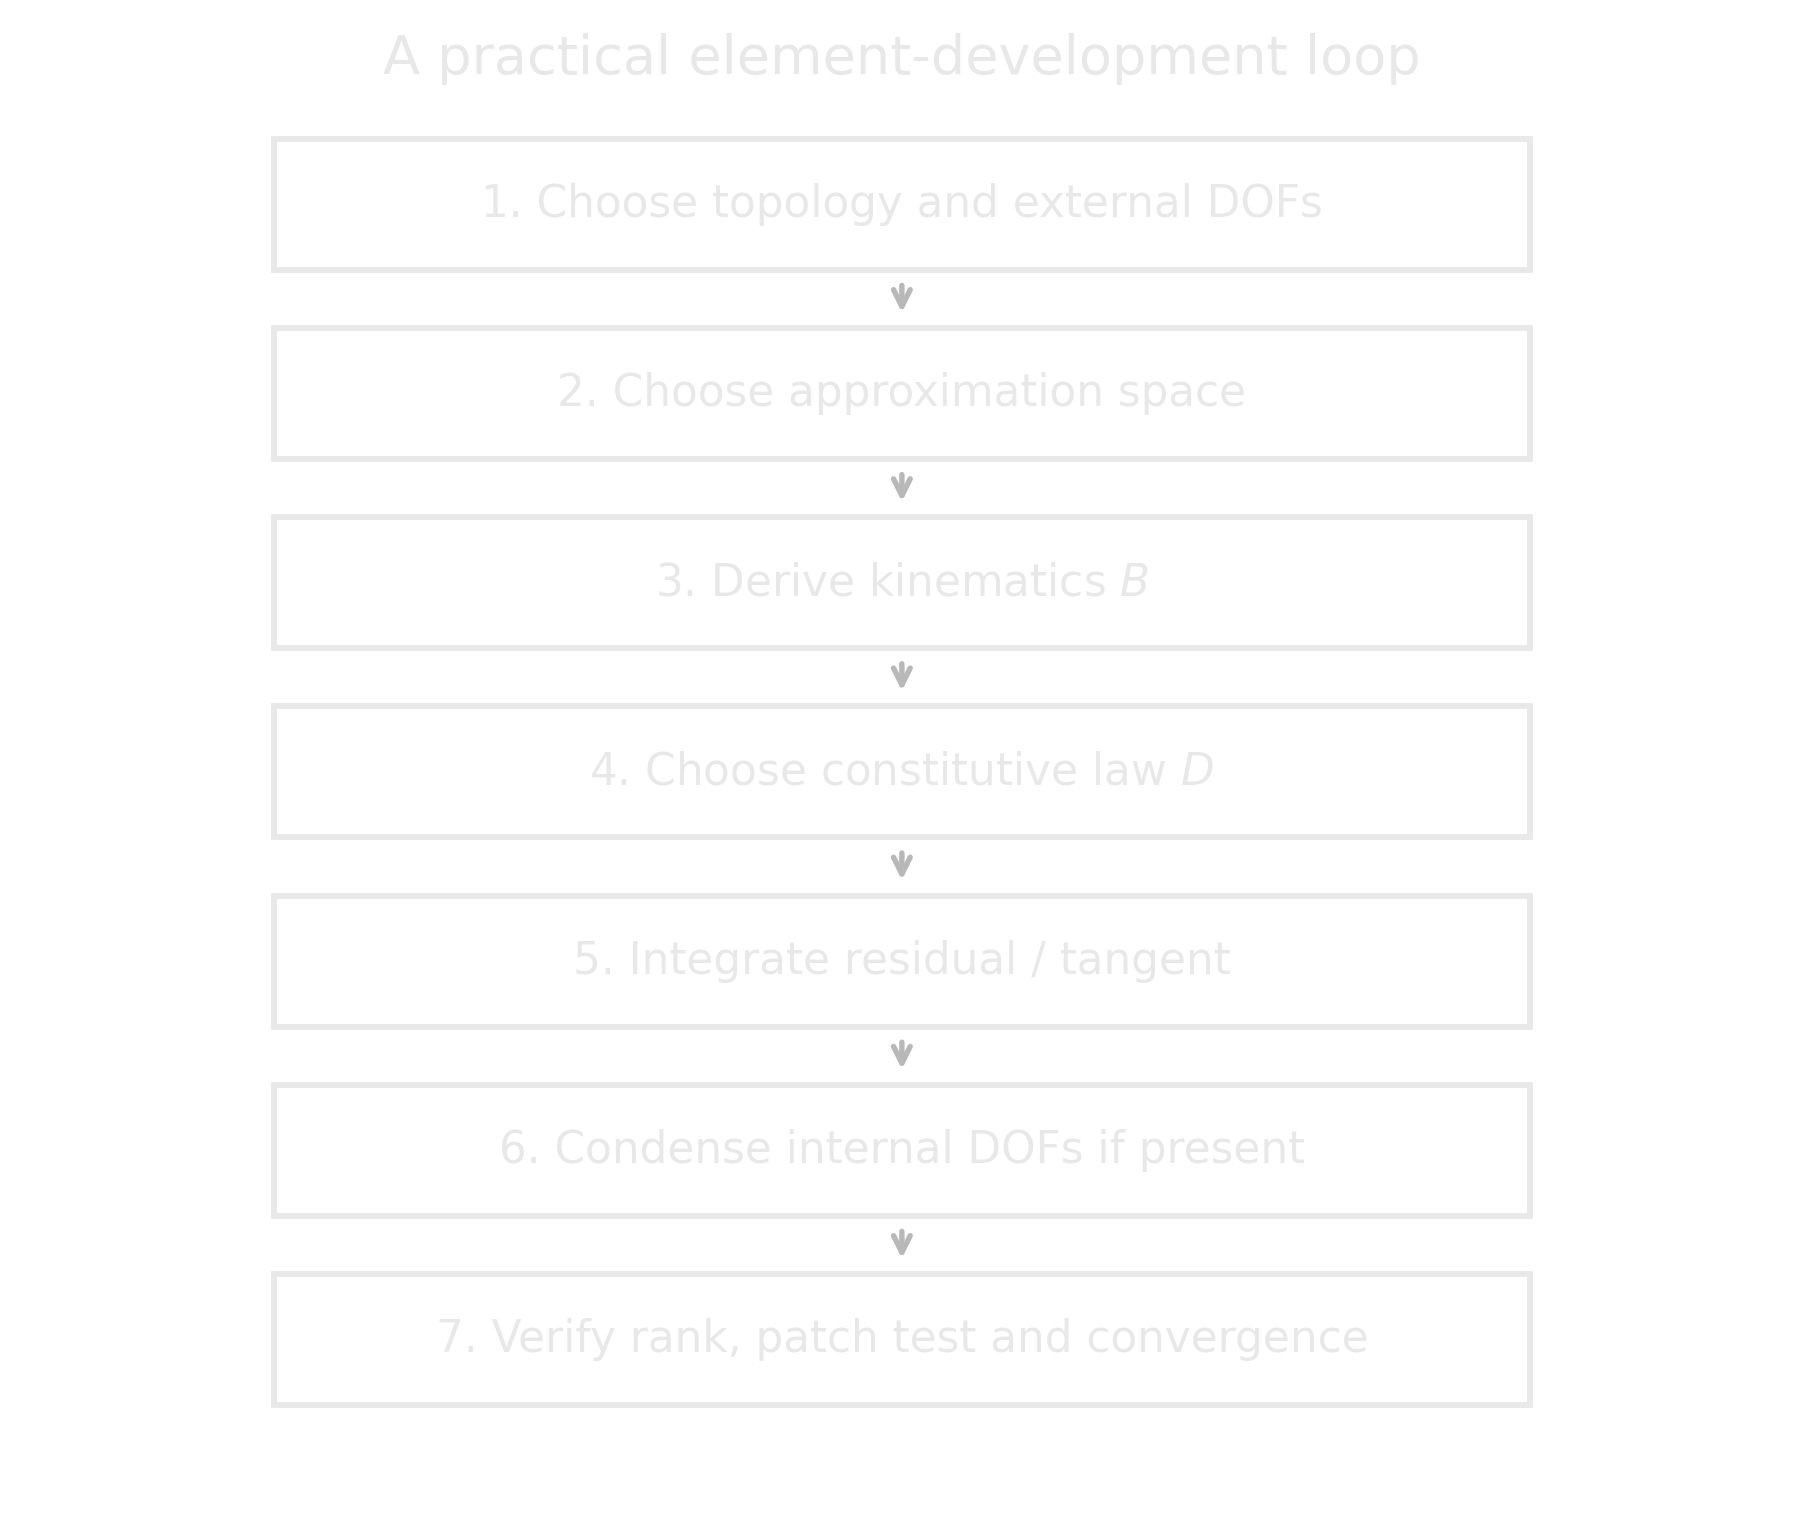
\includegraphics[width=0.72\textwidth]{img/fe_element_design_workflow.png}
    \caption{A practical development loop for a displacement-based finite
    element. The same logic extends to mixed, assumed-strain and enriched
    formulations, although additional fields and stability conditions enter.}
    \label{fig:fe-element-design-workflow}
\end{figure}

A useful checklist is:

\begin{enumerate}
    \item \textbf{Choose topology and external DOFs.} What information is shared
          with neighbouring elements and exposed to the global solver?
    \item \textbf{Choose the approximation space.} Which displacement, strain,
          stress or pressure fields should the element reproduce?
    \item \textbf{Derive the kinematics.} Construct $\m{B}$ or the corresponding
          nonlinear strain operator.
    \item \textbf{Choose the constitutive law.} Decide which physical stress or
          generalised force is work-conjugate to the chosen strain measure.
    \item \textbf{Choose integration.} The quadrature must represent the desired
          energy without introducing unintended constraints or zero-energy modes.
    \item \textbf{Introduce internal fields if needed.} Internal modes may enrich
          the approximation without adding global nodal DOFs.
    \item \textbf{Derive residual and tangent.} For nonlinear elements this is
          more fundamental than writing a closed-form stiffness matrix.
    \item \textbf{Verify before trusting.} Check rigid-body modes, constant-strain
          reproduction, patch tests, rank, symmetry when expected, convergence
          and sensitivity to distortion.
\end{enumerate}

The following examples show three different ways an engineer may change a
formulation. The first changes the interpolation or integration to avoid shear
locking. The second adds condensed internal quadratic modes to an eight-node
brick. The third keeps the continuum element itself unchanged and instead
changes the admissible discrete space through cyclic symmetry.

\section[Timoshenko Beam and Shear Locking]{Design Example I: Timoshenko Beam and Shear Locking}

The Timoshenko beam uses two independent kinematic fields: transverse
displacement $w(x)$ and section rotation $\varphi(x)$. With the sign convention
used here,

\begin{equation}
    \kappa=\varphi'(x),
    \qquad
    \gamma=w'(x)-\varphi(x).
\end{equation}

The bending and shear energies are

\begin{equation}
    U_b=\frac{1}{2}\int_0^LEI\kappa^2\,dx,
    \qquad
    U_s=\frac{1}{2}\int_0^Lk_sGA\gamma^2\,dx.
\end{equation}

A naive two-node element interpolates both fields linearly,

\begin{align}
    w(x)&=N_1w_1+N_2w_2,\\
    \varphi(x)&=N_1\varphi_1+N_2\varphi_2,
\end{align}

where

\begin{equation}
    N_1=1-\frac{x}{L},\qquad N_2=\frac{x}{L}.
\end{equation}

Then $w'$ is constant while $\varphi$ is linear. In pure bending the exact
kinematics can be written

\begin{equation}
    \varphi=\kappa x,
    \qquad
    w=\frac{1}{2}\kappa x^2,
\end{equation}

so that $\gamma=0$ everywhere. If only the end values of this field are supplied
to the two-node linear interpolation,

\begin{equation}
    w_1=0,
    \quad
    w_2=\frac{1}{2}\kappa L^2,
    \quad
    \varphi_1=0,
    \quad
    \varphi_2=\kappa L,
\end{equation}

then

\begin{equation}\label{eq:timo-spurious-shear}
    \boxed{
    \gamma^h(x)=\kappa\left(\frac{L}{2}-x\right)
    }.
\end{equation}

The discrete element therefore stores shear energy in a deformation that should
be pure bending. Integrating Equation~\eqref{eq:timo-spurious-shear} gives

\begin{equation}
    U_s^h
    =\frac{k_sGA\kappa^2L^3}{24},
\end{equation}

while the correct bending energy is

\begin{equation}
    U_b
    =\frac{EI\kappa^2L}{2}.
\end{equation}

Their ratio is

\begin{equation}\label{eq:timo-locking-ratio}
    \boxed{
    \frac{U_s^h}{U_b}
    =\frac{k_sGA L^2}{12EI}
    }.
\end{equation}

For a slender beam this ratio grows approximately with $(L/h)^2$. The element
therefore becomes artificially stiff precisely in the limit where shear
flexibility should become irrelevant. That is shear locking.

\begin{figure}[ht]
    \centering
    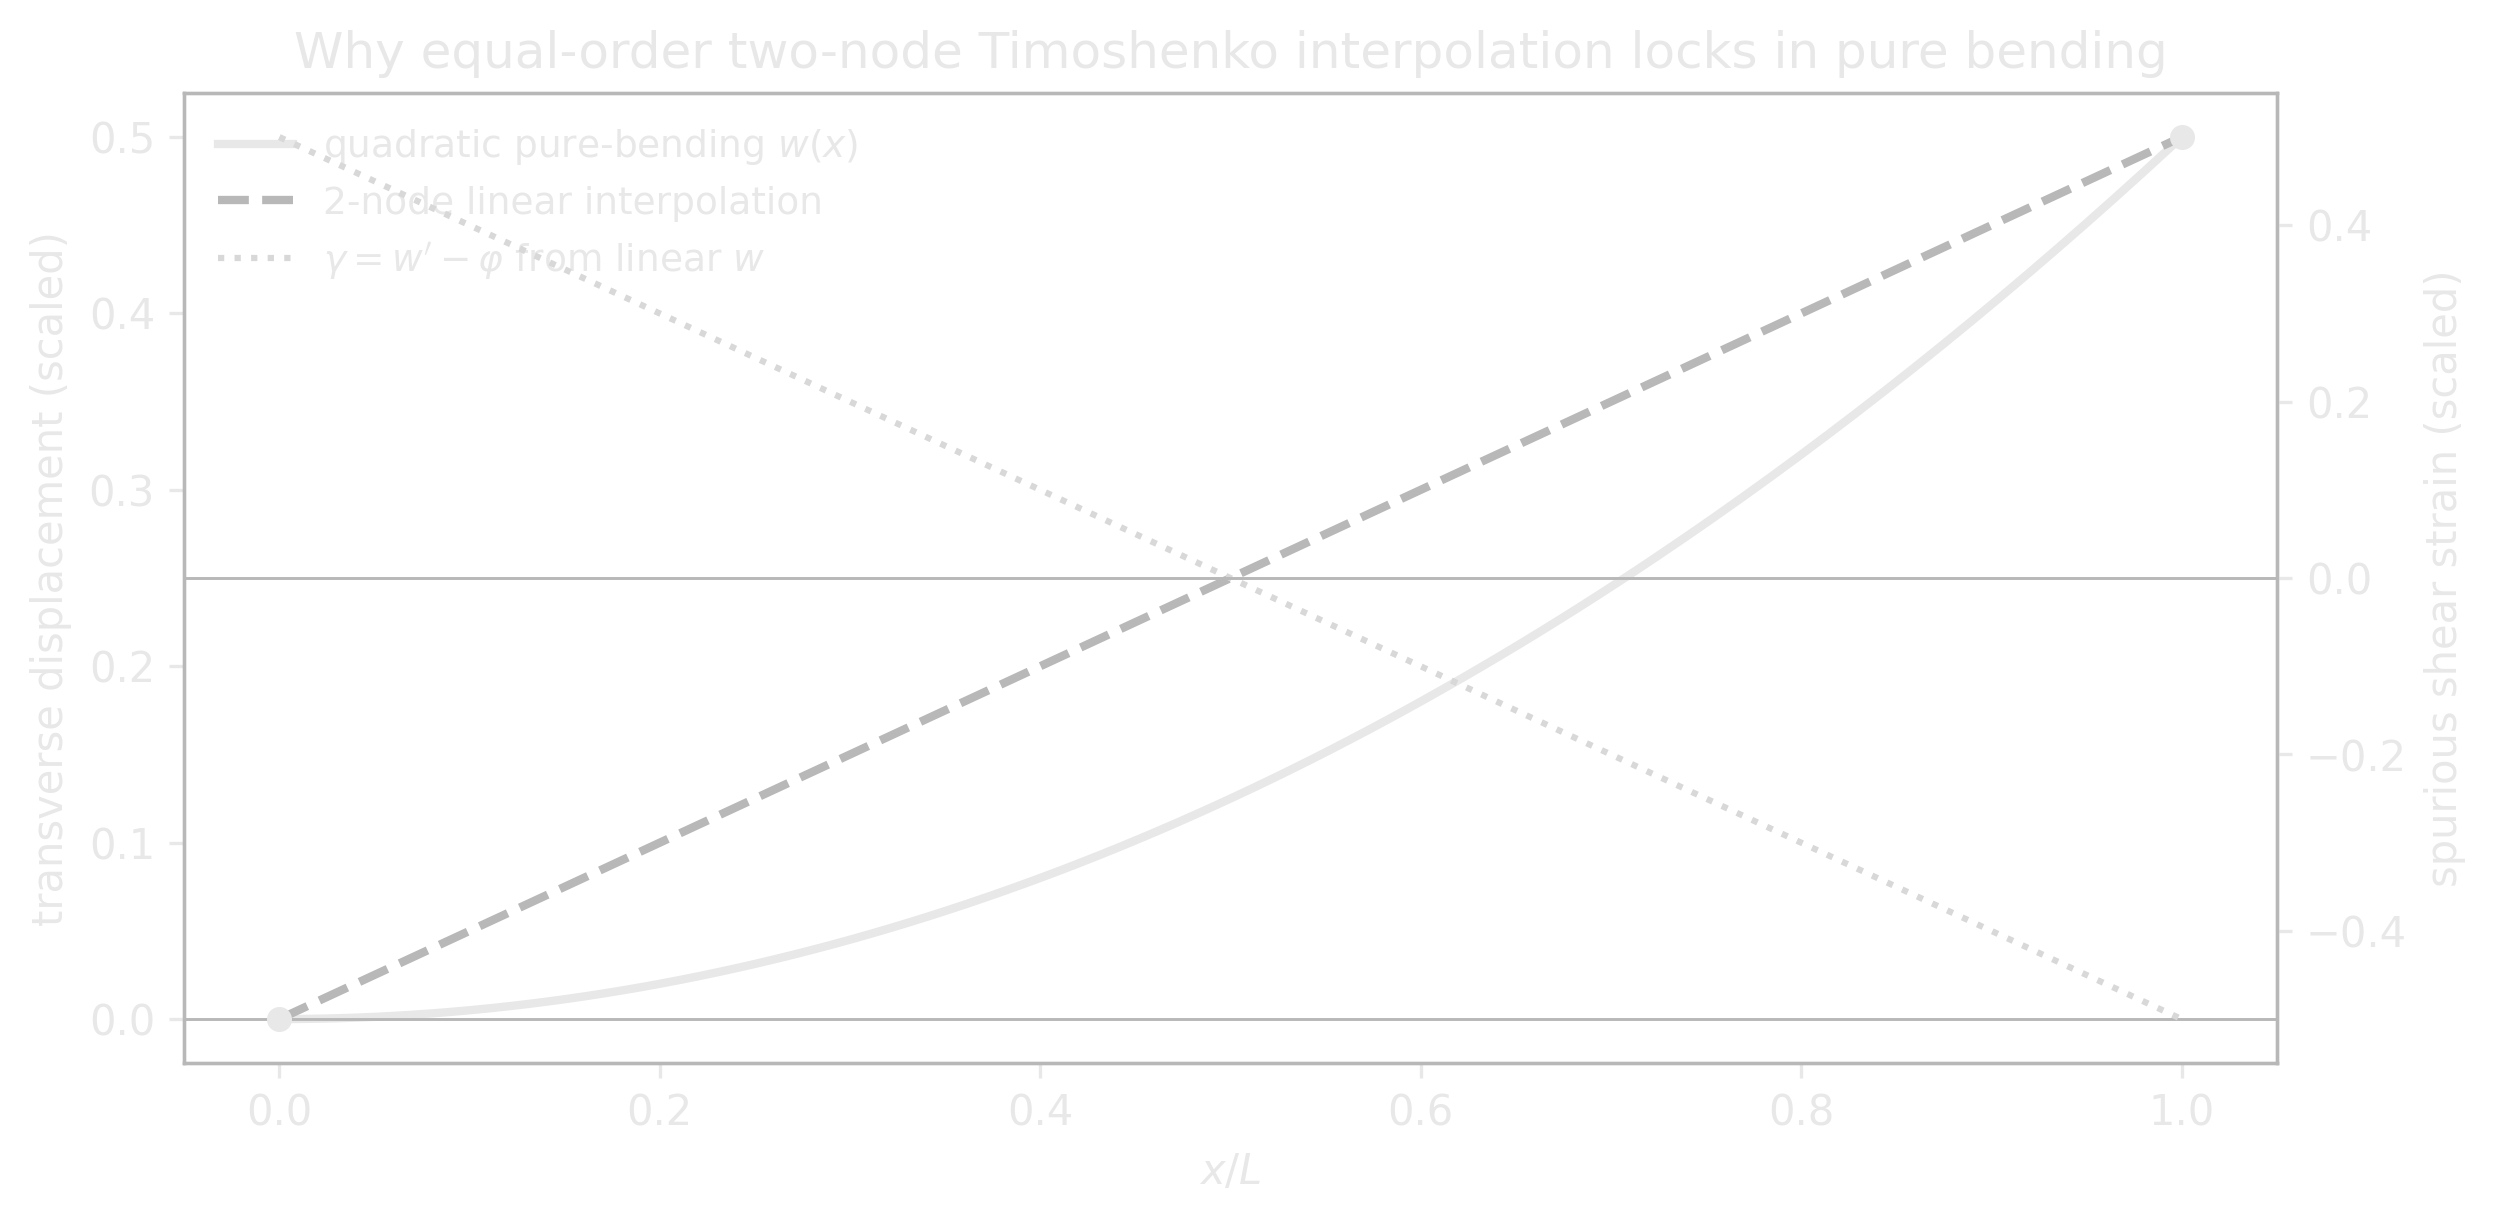
\includegraphics[width=0.88\textwidth]{img/fe_timoshenko_shear_locking.png}
    \caption{Pure bending requires a quadratic transverse displacement and a
    linear rotation. Equal-order linear interpolation of $w$ and $\varphi$
    cannot make $w'-\varphi$ vanish pointwise, producing a spurious shear field.}
    \label{fig:fe-timo-locking}
\end{figure}

\subsection{Three Different Remedies}

The important lesson is that locking is not caused by an incorrect continuum
law. It is caused by a discrete approximation that over-constrains the limiting
kinematics. Several remedies are therefore possible.

\paragraph{Compatible higher-order interpolation.}
Enrich $w$ so that $w'$ has the same polynomial order as $\varphi$. For example,
add an internal quadratic bubble coordinate $\alpha$,

\begin{equation}
    w(s)=N_1w_1+N_2w_2+\alpha s(1-s),
    \qquad s=\frac{x}{L}.
\end{equation}

For the pure-bending nodal data above, choosing

\begin{equation}
    \alpha=-\frac{1}{2}\kappa L^2
\end{equation}

recovers $w=\kappa x^2/2$ exactly and hence $\gamma=0$ everywhere. The internal
coordinate may be statically condensed so that the global element still has
only the usual nodal DOFs.

\paragraph{Reduced/selective integration.}
The linear interpolation gives $\gamma^h=0$ at the element centre $x=L/2$. If
the shear-energy term is evaluated with a single central integration point, the
spurious pure-bending shear energy vanishes. This is computationally cheap and
widely used, but underintegration must be checked for unintended zero-energy
modes.

\paragraph{Assumed or mixed shear field.}
Instead of accepting $\gamma=w'-\varphi$ pointwise, construct an assumed shear
strain or introduce shear force/strain as an independent field. MITC, assumed
natural strain and related formulations use this general idea in beams, plates
and shells.

\begin{notebooknote}[General lesson -- Locking is a discrete-space problem]

Shear locking, volumetric locking and many parasitic strain modes are best
understood by asking whether the chosen interpolation can reproduce the
constraint that should hold in the limiting physical case. More Gauss points do
not repair a bad approximation space; they may enforce its defect more exactly.
\end{notebooknote}

\subsection{Executable Shear-Locking Check}

The following function evaluates the shear energy of the naive element for the
pure-bending nodal state and compares it with the bending energy. It also shows
why one-point shear integration eliminates this particular parasitic mode.

\begin{python}
def timoshenko_pure_bending_check(L, EI, kGA, curvature):
    # Nodal data sampled from the exact pure-bending field.
    w1 = 0.0
    w2 = 0.5 * curvature * L * L
    phi1 = 0.0
    phi2 = curvature * L

    # Exact integral of gamma^2 for the equal-order linear interpolation.
    shear_energy_full = kGA * curvature**2 * L**3 / 24.0
    bending_energy = EI * curvature**2 * L / 2.0

    # One-point shear integration at x=L/2.
    x = 0.5 * L
    dw_dx = (w2 - w1) / L
    phi = 0.5 * phi1 + 0.5 * phi2
    gamma_center = dw_dx - phi
    shear_energy_reduced = 0.5 * kGA * gamma_center**2 * L

    # Internal quadratic mode required for exact pure bending.
    alpha = -0.5 * curvature * L * L

    return {
        "full_shear_energy": shear_energy_full,
        "bending_energy": bending_energy,
        "energy_ratio": shear_energy_full / bending_energy,
        "reduced_shear_energy": shear_energy_reduced,
        "bubble_alpha": alpha,
    }


result = timoshenko_pure_bending_check(
    L=100.0,
    EI=2.0e8,
    kGA=8.0e5,
    curvature=1.0e-4,
)
for key, value in result.items():
    print(key, value)
\end{python}

The numerical values are secondary. The important result is that the full
integration stores a nonzero shear energy, the one-point shear evaluation sees
zero shear at the centre, and the required higher-order internal coordinate is
computed directly from the missing quadratic deformation.

\section[Building an Eight-Node Brick]{Design Example II: Building an Eight-Node\\Brick}

The next example develops the core of a three-dimensional solid element and then
adds internal quadratic enrichment. This is deliberately more general than a
catalogue entry: it shows which pieces of code have to exist for almost any
isoparametric continuum element.

\subsection{Trilinear HEX8 Interpolation}

Let the eight corner nodes have natural coordinates

\begin{equation}
    (\xi_i,\eta_i,\zeta_i)\in\{-1,+1\}^3.
\end{equation}

The standard trilinear shape functions are

\begin{equation}\label{eq:hex8-shape}
    \boxed{
    N_i(\xi,\eta,\zeta)
    =\frac{1}{8}
    (1+\xi_i\xi)
    (1+\eta_i\eta)
    (1+\zeta_i\zeta)
    }.
\end{equation}

The displacement approximation contains 24 external DOFs,

\begin{equation}
    \m{q}_e
    =
    \begin{bmatrix}
        u_1&v_1&w_1&\cdots&u_8&v_8&w_8
    \end{bmatrix}^T.
\end{equation}

At each integration point, Equation~\eqref{eq:hex8-shape} generates the Jacobian,
physical shape-function gradients and finally the $6\times24$ matrix $\m{B}$.

\subsection{A Reusable HEX8 Kernel}

\begin{python}
HEX8_SIGNS = np.array([
    [-1, -1, -1],
    [ 1, -1, -1],
    [ 1,  1, -1],
    [-1,  1, -1],
    [-1, -1,  1],
    [ 1, -1,  1],
    [ 1,  1,  1],
    [-1,  1,  1],
], dtype=float)


def hex8_shape_values(xi, eta, zeta):
    N = np.zeros(8, dtype=float)
    for n, (sx, sy, sz) in enumerate(HEX8_SIGNS):
        N[n] = 0.125 * (1.0 + sx*xi) * (1.0 + sy*eta) * (1.0 + sz*zeta)
    return N


def hex8_shape_derivatives(xi, eta, zeta):
    dN = np.zeros((8, 3), dtype=float)
    for n, (sx, sy, sz) in enumerate(HEX8_SIGNS):
        dN[n, 0] = 0.125 * sx * (1.0 + sy*eta) * (1.0 + sz*zeta)
        dN[n, 1] = 0.125 * sy * (1.0 + sx*xi) * (1.0 + sz*zeta)
        dN[n, 2] = 0.125 * sz * (1.0 + sx*xi) * (1.0 + sy*eta)
    return dN


def build_solid_B(dN_dx):
    B = np.zeros((6, 24), dtype=float)
    for n, (Nx, Ny, Nz) in enumerate(dN_dx):
        c = 3*n
        B[0, c    ] = Nx
        B[1, c + 1] = Ny
        B[2, c + 2] = Nz
        B[3, c    ] = Ny
        B[3, c + 1] = Nx
        B[4, c + 1] = Nz
        B[4, c + 2] = Ny
        B[5, c    ] = Nz
        B[5, c + 2] = Nx
    return B


def isotropic_D(E, nu):
    c = E / ((1.0 + nu) * (1.0 - 2.0*nu))
    return c * np.array([
        [1-nu, nu, nu, 0, 0, 0],
        [nu, 1-nu, nu, 0, 0, 0],
        [nu, nu, 1-nu, 0, 0, 0],
        [0, 0, 0, (1-2*nu)/2, 0, 0],
        [0, 0, 0, 0, (1-2*nu)/2, 0],
        [0, 0, 0, 0, 0, (1-2*nu)/2],
    ], dtype=float)


def hex8_stiffness(node_xyz, E, nu):
    D = isotropic_D(E, nu)
    Ke = np.zeros((24, 24), dtype=float)
    a = 1.0 / math.sqrt(3.0)

    for xi in (-a, a):
        for eta in (-a, a):
            for zeta in (-a, a):
                dN_dxi = hex8_shape_derivatives(xi, eta, zeta)

                # J = dx/dxi.  node_xyz is 8x3, dN_dxi is 8x3.
                J = node_xyz.T @ dN_dxi
                Jinv, detJ = inverse_3x3(J)
                if detJ <= 0.0:
                    raise ValueError("non-positive HEX8 Jacobian")

                dN_dx = dN_dxi @ Jinv
                B = build_solid_B(dN_dx)
                Ke += B.T @ D @ B * detJ

    return Ke
\end{python}

The code is the direct algorithmic expansion of

\begin{equation}
    \m{K}_e
    =\int\m{B}^T\m{D}\m{B}\,d\Omega.
\end{equation}

There is no hidden ``HEX8 stiffness formula.'' The element is a loop that
constructs a local interpolation derivative, maps it to physical space,
evaluates the constitutive energy and accumulates the result.

\section[Quadratic Internal Enrichment of HEX8]{Design Example III: Quadratic Internal\\Enrichment of HEX8}

A conventional eight-node brick is trilinear in its external nodal
interpolation. Calling it a ``quadratic eight-node brick'' without qualification
would therefore be misleading. It is nevertheless possible to keep the eight
external corner nodes while introducing additional \textit{internal} polynomial
coordinates that are eliminated before global assembly.

This idea is useful for understanding incompatible-mode and enhanced-strain
elements. The following formulation is educational rather than a recommendation
for a production brick, but it exposes the design mechanism clearly.

\begin{figure}[ht]
    \centering
    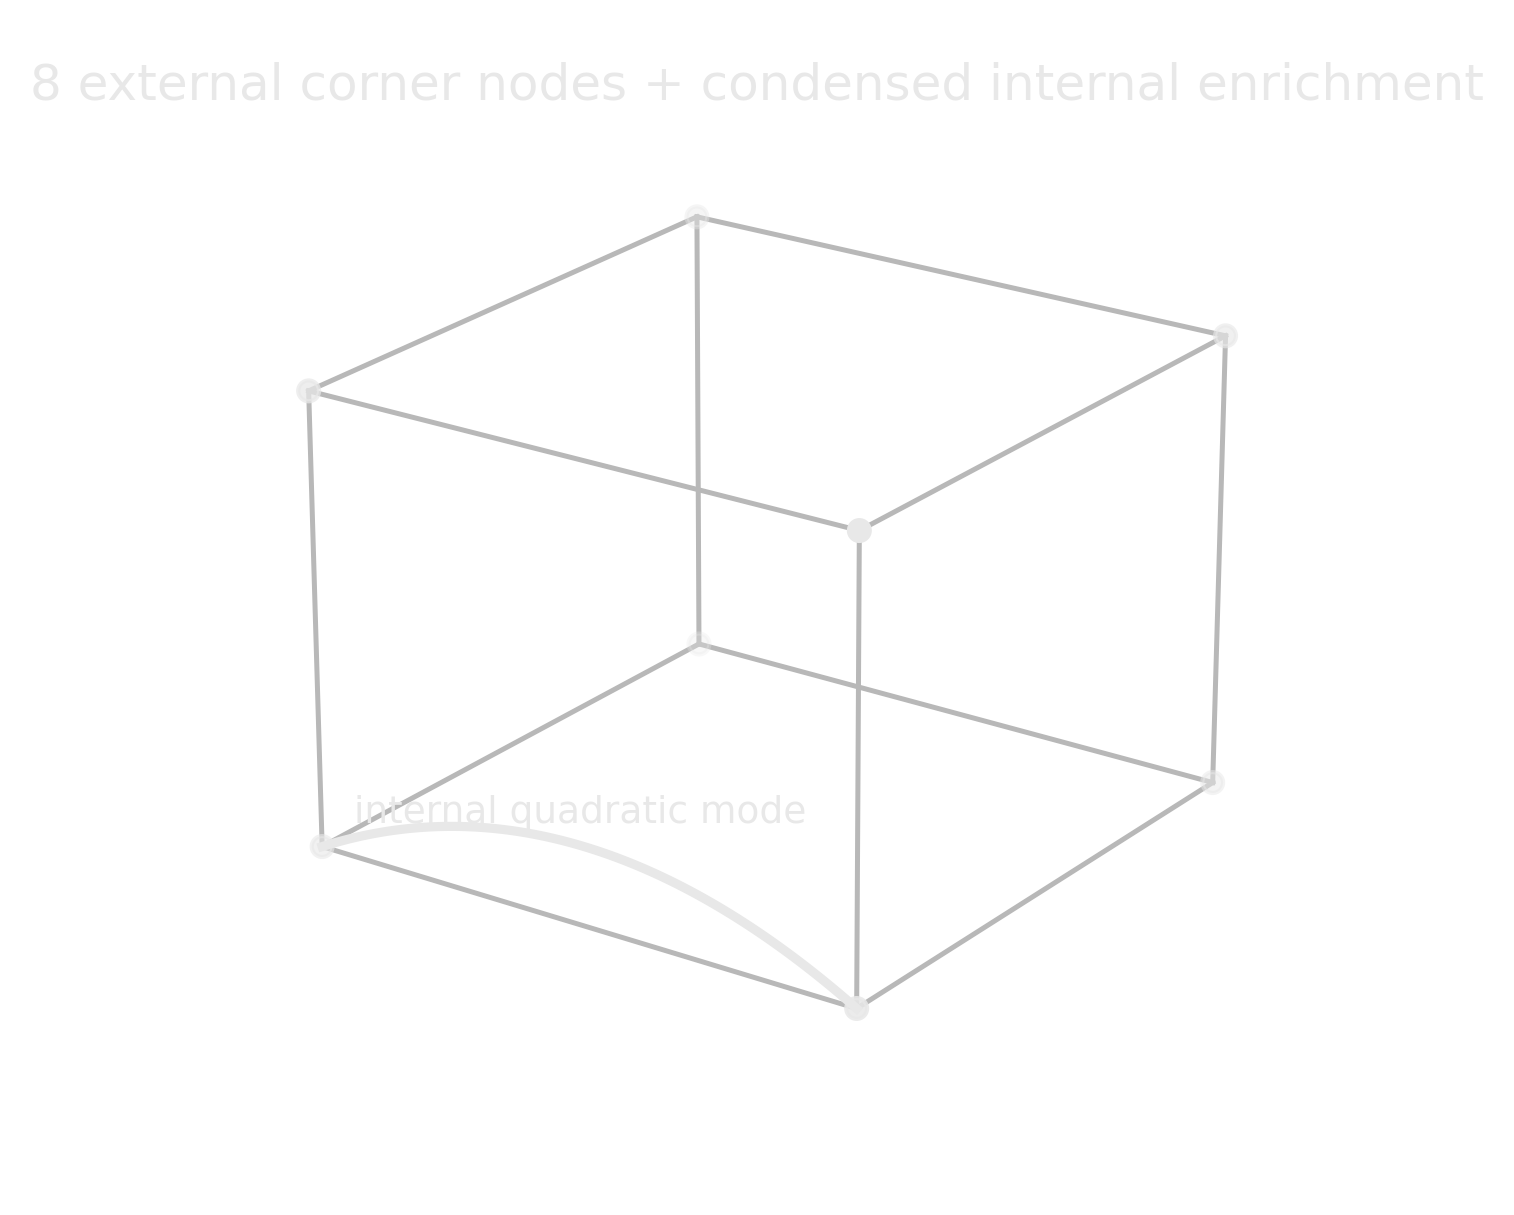
\includegraphics[width=0.60\textwidth]{img/fe_enriched_hex8.png}
    \caption{An element may retain eight external corner nodes while using
    additional internal deformation coordinates. If the internal coordinates
    are condensed locally, the global solver still sees only the original 24
    nodal DOFs.}
    \label{fig:fe-enriched-hex8}
\end{figure}

\subsection{Add Internal Quadratic Modes}

Augment the displacement field as

\begin{equation}\label{eq:enriched-displacement}
    \boxed{
    \m{u}^h
    =\m{N}_q\m{q}
    +\m{N}_{\alpha}\M{\alpha}
    }.
\end{equation}

The external coordinates $\m{q}$ are the 24 corner-node displacements. The
internal coordinates $\M{\alpha}$ are not shared between elements. As a simple
quadratic enrichment in natural coordinates, define

\begin{equation}
    \psi_1=1-\xi^2,
    \qquad
    \psi_2=1-\eta^2,
    \qquad
    \psi_3=1-\zeta^2,
\end{equation}

and allow each displacement component to contain these three modes. There are
therefore nine internal coordinates.

These modes vanish at all eight corner nodes, so they do not alter the external
nodal values. They do not, however, vanish over all element faces. The element
is therefore an \textit{incompatible displacement enrichment}; neighbouring
elements need not share the same internal field on their common face. A
production incompatible-mode formulation must be designed and verified so that
this nonconformity does not destroy patch-test consistency.

The strain is

\begin{equation}
    \M{\varepsilon}
    =\m{B}_q\m{q}
    +\m{B}_{\alpha}\M{\alpha}.
\end{equation}

Virtual work gives the local system

\begin{equation}\label{eq:enriched-block-system}
    \begin{bmatrix}
        \m{K}_{qq} & \m{K}_{q\alpha}\\
        \m{K}_{\alpha q} & \m{K}_{\alpha\alpha}
    \end{bmatrix}
    \begin{bmatrix}
        \m{q}\\
        \M{\alpha}
    \end{bmatrix}
    =
    \begin{bmatrix}
        \m{f}_q\\
        \m{0}
    \end{bmatrix}.
\end{equation}

Because the internal coordinates have no external nodal force, their equilibrium
requires

\begin{equation}
    \m{K}_{\alpha q}\m{q}
    +\m{K}_{\alpha\alpha}\M{\alpha}=\m{0},
\end{equation}

hence

\begin{equation}
    \M{\alpha}
    =-\m{K}_{\alpha\alpha}^{-1}
    \m{K}_{\alpha q}\m{q}.
\end{equation}

Substitution into the external equilibrium gives the condensed stiffness

\begin{equation}\label{eq:enriched-condensed-stiffness}
    \boxed{
    \m{K}_{e}
    =\m{K}_{qq}
    -\m{K}_{q\alpha}
     \m{K}_{\alpha\alpha}^{-1}
     \m{K}_{\alpha q}
    }.
\end{equation}

This is exactly the same algebraic operation that later appears in static
condensation and model reduction. The difference is interpretation: here the
eliminated coordinates are part of the \textit{element formulation itself} and
never become global model DOFs.

\subsection{Why the Quadratic Mode Helps in Bending}

Consider a unit brick subjected to the small-strain pure-bending displacement
field

\begin{equation}\label{eq:hex-pure-bending-field}
    u=-\kappa xz,
    \qquad
    v=0,
    \qquad
    w=\frac{1}{2}\kappa x^2.
\end{equation}

Then

\begin{equation}
    \varepsilon_{xx}=-\kappa z,
    \qquad
    \gamma_{xz}=u_{,z}+w_{,x}=0.
\end{equation}

At the eight corner nodes $x=\pm1$, however,

\begin{equation}
    w_i=\frac{1}{2}\kappa
\end{equation}

is the same at every corner. The standard trilinear HEX8 therefore reconstructs
this part of the nodal field as a constant translation and misses the interior
$x^2$ variation. Its reconstructed $w_{,x}=0$, producing the parasitic shear

\begin{equation}
    \gamma_{xz}^h=-\kappa x.
\end{equation}

The internal mode $\psi_1=1-\xi^2$ in the $w$ component can recover the missing
quadratic field. Taking

\begin{equation}
    \alpha_{w,1}=-\frac{1}{2}\kappa
\end{equation}

adds

\begin{equation}
    -\frac{1}{2}\kappa(1-x^2)
\end{equation}

to the constant corner interpolation and reproduces
$w=\kappa x^2/2$ exactly for this regular unit mapping.

This example parallels the Timoshenko beam: a parasitic shear appears because
the discrete displacement space cannot represent the limiting bending
kinematics. An internal higher-order mode supplies the missing deformation
without requiring additional external nodes.

\subsection{Implementation and Static Condensation}

\begin{python}
def internal_mode_derivatives(xi, eta, zeta):
    # Rows correspond to psi1=1-xi^2, psi2=1-eta^2, psi3=1-zeta^2.
    return np.array([
        [-2.0*xi, 0.0, 0.0],
        [0.0, -2.0*eta, 0.0],
        [0.0, 0.0, -2.0*zeta],
    ], dtype=float)


def build_internal_B(dpsi_dx):
    # 9 internal DOFs: 3 modes for u, then 3 for v, then 3 for w.
    B = np.zeros((6, 9), dtype=float)
    for m, (px, py, pz) in enumerate(dpsi_dx):
        iu = m
        iv = 3 + m
        iw = 6 + m

        B[0, iu] = px
        B[1, iv] = py
        B[2, iw] = pz
        B[3, iu] = py
        B[3, iv] = px
        B[4, iv] = pz
        B[4, iw] = py
        B[5, iu] = pz
        B[5, iw] = px
    return B


def enriched_hex8_stiffness(node_xyz, E, nu):
    D = isotropic_D(E, nu)
    Kqq = np.zeros((24, 24), dtype=float)
    Kqa = np.zeros((24, 9), dtype=float)
    Kaa = np.zeros((9, 9), dtype=float)
    a = 1.0 / math.sqrt(3.0)

    for xi in (-a, a):
        for eta in (-a, a):
            for zeta in (-a, a):
                dN_dxi = hex8_shape_derivatives(xi, eta, zeta)
                J = node_xyz.T @ dN_dxi
                Jinv, detJ = inverse_3x3(J)
                if detJ <= 0.0:
                    raise ValueError("non-positive HEX8 Jacobian")

                Bq = build_solid_B(dN_dxi @ Jinv)
                dpsi_dx = internal_mode_derivatives(xi, eta, zeta) @ Jinv
                Ba = build_internal_B(dpsi_dx)

                Kqq += Bq.T @ D @ Bq * detJ
                Kqa += Bq.T @ D @ Ba * detJ
                Kaa += Ba.T @ D @ Ba * detJ

    # X = Kaa^{-1} Kaq, but solved without forming an explicit inverse.
    X = solve_dense(Kaa, Kqa.T)
    Kcondensed = Kqq - Kqa @ X
    return Kcondensed, Kqq, Kqa, Kaa


# Regular cube with physical coordinates equal to natural corner coordinates.
cube = HEX8_SIGNS.copy()
K_enriched, K_standard, Kqa, Kaa = enriched_hex8_stiffness(
    cube, E=210000.0, nu=0.3
)

print("standard K[0,0] =", K_standard[0, 0])
print("enriched K[0,0] =", K_enriched[0, 0])
\end{python}

For the regular cube in the example, the selected diagonal term decreases after
condensation. That number by itself is not an element-quality measure, but it
illustrates an important energy property: allowing an internal field can only
relax, not artificially add, the energy associated with the constrained
external displacement state when the internal block is stable.

\begin{bbox}
\textbf{Engineering caution -- An enrichment is not automatically a good element.}

Adding polynomial modes can introduce rank deficiency, nonconforming interfaces,
poor distortion behaviour or spurious zero-energy states. A useful enrichment
must be justified by the intended limiting kinematics and then verified with
patch tests and convergence studies. Production incompatible-mode bricks use
carefully selected enhancement fields; the simple modes above are intended to
show the derivation mechanism, not to replace such formulations.
\end{bbox}



\section[Rotation-Enriched Eight-Node Brick]{Design Example IV: Rotation-Enriched\\Eight-Node Brick}\label{sec:hex8-nodal-rotations}

The preceding enriched HEX8 introduced higher-order deformation through local
coordinates that were condensed before assembly.  Another possibility is to
expose part of the higher-order information as nodal slope or rotation
coordinates.  The engineering objective considered here is very specific:

\begin{quote}
Can an eight-corner brick be made substantially richer in bending and twisting
so that rotating one corner changes the displacement field inside the element,
without interpreting that rotation as a new material degree of freedom?
\end{quote}

The answer is yes.  A useful way to understand such a formulation is to start
from the ordinary 20-node quadratic hexahedron.  It has 20 nodes with three
translations each,

\begin{equation}
    \m{q}_{20}\in\mathbb{R}^{60}.
\end{equation}

Keep the eight corner translations but replace the twelve midside-node
translations by three slope/rotation parameters at each corner,

\begin{equation}
    \m{q}_{48}
    =
    \begin{bmatrix}
        u_1&v_1&w_1&\theta_{x1}&\theta_{y1}&\theta_{z1}&\cdots&
        u_8&v_8&w_8&\theta_{x8}&\theta_{y8}&\theta_{z8}
    \end{bmatrix}^{T}.
\end{equation}

The element then still has only eight visible geometric nodes, but its
displacement interpolation is inherited from a quadratic 20-node solid.

\subsection{The Edge Relation: Translation and Slope Replace a Midside Node}

Consider one edge from corner $i$ to corner $j$ with

\begin{equation}
    \m{l}_{ij}=\m{x}_j-\m{x}_i,
    \qquad L_{ij}=\lVert\m{l}_{ij}\rVert,
    \qquad \m{t}_{ij}=\frac{\m{l}_{ij}}{L_{ij}}.
\end{equation}

For a scalar transverse displacement $w(s)$, cubic Hermite interpolation on
$0\le s\le L$ gives at the midpoint

\begin{equation}\label{eq:hermite-midpoint}
    \boxed{
    w_m
    =\frac{w_i+w_j}{2}
    +\frac{L}{8}(\theta_i-\theta_j)
    }.
\end{equation}

The first term is the ordinary linear midpoint displacement.  The second term
contains the missing curvature information.  In three dimensions a small
rotation produces the edge slope

\begin{equation}
    \frac{\partial\m{u}}{\partial s}
    =\M{\theta}\times\m{t}_{ij}.
\end{equation}

Equation~\eqref{eq:hermite-midpoint} therefore becomes

\begin{equation}\label{eq:rot-hex-midpoint}
    \boxed{
    \m{u}_m
    =\frac{1}{2}(\m{u}_i+\m{u}_j)
    +\frac{1}{8}(\M{\theta}_i-\M{\theta}_j)\times\m{l}_{ij}
    }.
\end{equation}

A rotation parallel to the edge produces no edge displacement, as expected.
Rotations about the other two directions move the midside point transversely
and thereby introduce bending information that a corner-translation-only HEX8
does not possess.

\begin{figure}[ht]
    \centering
    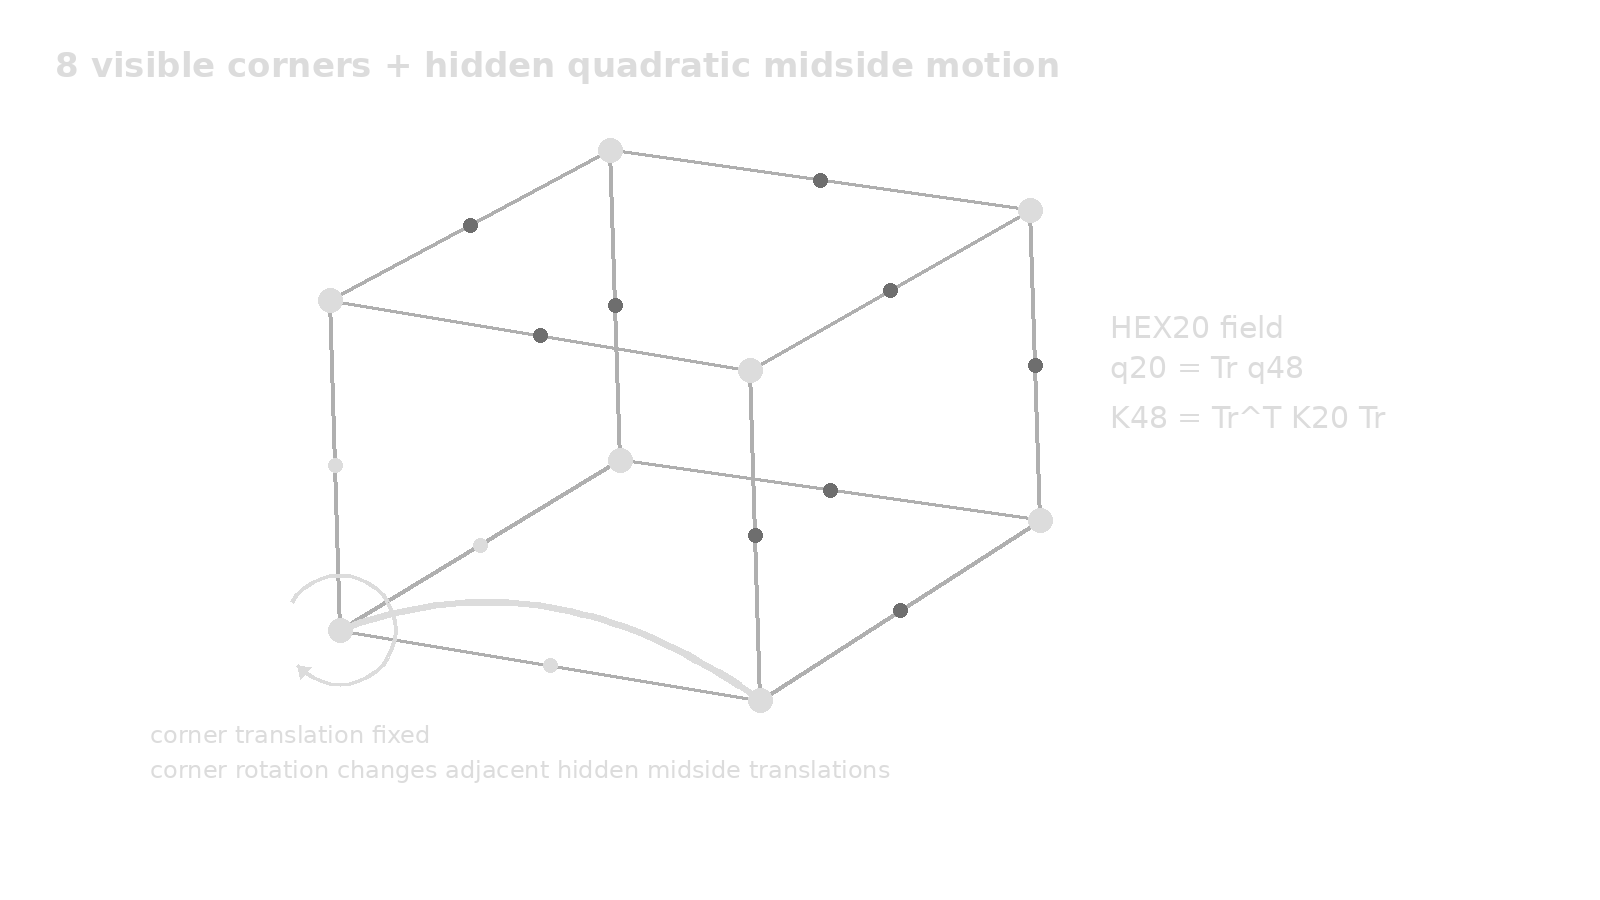
\includegraphics[width=0.78\textwidth]{img/fe_rotation_enriched_hex8.png}
    \caption{Concept of the rotation-enriched brick.  The visible mesh contains
    only eight corner nodes.  Corner translations and rotations generate the
    twelve hidden midside translations of a quadratic HEX20 interpolation.
    Rotating one corner therefore changes the internal displacement field even
    if the corner translation is fixed.}
    \label{fig:rotation-enriched-hex8}
\end{figure}

\subsection{Transformation from 48 to 60 Coordinates}

Collect Equation~\eqref{eq:rot-hex-midpoint} for the twelve edges.  Corner
translations are copied directly and hidden midside translations are generated
from the adjacent corners.  This defines

\begin{equation}\label{eq:rot-hex-transform}
    \boxed{
    \m{q}_{20}=\m{T}_{r}\m{q}_{48}
    },
    \qquad
    \m{T}_{r}\in\mathbb{R}^{60\times48}.
\end{equation}

For edge $(i,j)$ the $3\times48$ block corresponding to its midside node contains

\begin{equation}
    \m{T}_{m,i}^{(u)}=\frac12\m{I},
    \qquad
    \m{T}_{m,j}^{(u)}=\frac12\m{I},
\end{equation}

and, using the skew matrix $[\m{l}]_{\times}\m{a}=\m{l}\times\m{a}$,

\begin{equation}
    \m{T}_{m,i}^{(\theta)}=-\frac18[\m{l}_{ij}]_{\times},
    \qquad
    \m{T}_{m,j}^{(\theta)}= \frac18[\m{l}_{ij}]_{\times}.
\end{equation}

The ordinary quadratic-brick displacement field

\begin{equation}
    \m{u}^{h}=\m{N}_{20}\m{q}_{20}
\end{equation}

can therefore be written directly in the visible coordinates,

\begin{equation}
    \boxed{
    \m{u}^{h}=\m{N}_{20}\m{T}_{r}\m{q}_{48}
    }.
\end{equation}

The rotations are thus \emph{parameters of an ordinary Cauchy displacement
field}; no couple stresses or microrotation material constants are introduced.

If the 20-node stiffness and mass are

\begin{equation}
    \m{K}_{20}
    =\int\m{B}_{20}^{T}\m{D}\m{B}_{20}\,d\Omega,
    \qquad
    \m{M}_{20}
    =\int\rho\m{N}_{20}^{T}\m{N}_{20}\,d\Omega,
\end{equation}

virtual work gives immediately

\begin{equation}\label{eq:rot-hex-km}
    \boxed{
    \m{K}_{48}=\m{T}_{r}^{T}\m{K}_{20}\m{T}_{r},
    \qquad
    \m{M}_{48}=\m{T}_{r}^{T}\m{M}_{20}\m{T}_{r}
    }.
\end{equation}

This is exactly the same congruence principle already encountered for
constraints and reduced coordinates in Chapters~\ref{chap:multifreedom-constraints}
and~\ref{chap:kinematic-constraints}.

\subsection{Why a Corner Twist Changes the Interior Field}

Set every coordinate to zero except, for example,

\begin{equation}
    \theta_{z1}=\Theta.
\end{equation}

The corner displacement remains zero, but every hidden midside node on an edge
meeting node~1 receives a transverse displacement according to
Equation~\eqref{eq:rot-hex-midpoint}.  The quadratic HEX20 shape functions then
carry that information across the complete element volume.  The rotational DOF
therefore acts much like the slope DOF of a Hermite beam: it controls a
higher-order displacement field between the geometric nodes.

This is the reason such an element may represent bending or twisting with fewer
geometric elements than a low-order translational brick.  The relevant measure
is not DOFs per element but total DOFs required to achieve the desired accuracy.

\subsection{An Important Stability Caveat}

Equation~\eqref{eq:rot-hex-midpoint} is an intuitive Hermite construction, but
it also exposes a general difficulty of rotational solids: the mapping from
corner rotations to midside translations need not make every rotational
combination energetically visible.  Additional zero-energy rotational patterns
can remain.  Established 48-DOF hexahedral formulations therefore supplement
the transformed quadratic field with carefully designed stabilization or
penalty terms and must be checked for patch-test consistency and rank.

This is not a defect of the idea; it is an excellent example of why element
design cannot stop after writing richer shape functions.  The complete
formulation is

\begin{equation}
    \boxed{
    \text{approximation space}
    +\text{energy}
    +\text{integration}
    +\text{stabilization}
    +\text{verification}
    }.
\end{equation}

\begin{bbox}
\textbf{Do not confuse this rotation with a micropolar rotation.}

Here $\M{\theta}$ is a slope-like coordinate used to parameterize an ordinary
Cauchy displacement interpolation.  A micropolar solid instead introduces an
independent material rotation field and couple stresses.  Both may expose six
numbers per node, but their continuum physics is different.
\end{bbox}

\subsection{Executable Transformation Builder}

The following code constructs the 60-by-48 transformation and demonstrates the
response to a single corner twist.  It deliberately stops before adding a
production stabilization law; the resulting rank check belongs to the element
verification stage.

\begin{python}
HEX8_EDGES = (
    (0, 1), (1, 2), (2, 3), (3, 0),
    (4, 5), (5, 6), (6, 7), (7, 4),
    (0, 4), (1, 5), (2, 6), (3, 7),
)


def skew_matrix(v):
    x, y, z = v
    return np.array([
        [0.0, -z,   y],
        [z,    0.0, -x],
        [-y,   x,   0.0],
    ], dtype=float)


def rotation_enriched_hex8_transform(corner_xyz):
    T = np.zeros((60, 48), dtype=float)

    # HEX20 corner translations are the visible corner translations.
    for i in range(8):
        T[3*i:3*i+3, 6*i:6*i+3] = np.eye(3)

    # Hidden HEX20 midside translations follow the Hermite midpoint relation.
    for edge, (i, j) in enumerate(HEX8_EDGES):
        row = 3 * (8 + edge)
        l = corner_xyz[j] - corner_xyz[i]

        T[row:row+3, 6*i:6*i+3] = 0.5 * np.eye(3)
        T[row:row+3, 6*j:6*j+3] = 0.5 * np.eye(3)

        T[row:row+3, 6*i+3:6*i+6] = -skew_matrix(l) / 8.0
        T[row:row+3, 6*j+3:6*j+6] =  skew_matrix(l) / 8.0

    return T


cube = HEX8_SIGNS.copy()
Trot = rotation_enriched_hex8_transform(cube)

q48 = np.zeros(48, dtype=float)
q48[5] = 0.10              # theta_z at corner 1
q20 = Trot @ q48

print("hidden midside translations on the 12 edges:")
print(q20[24:].reshape((12, 3)))
\end{python}

The nonzero hidden midside translations are the discrete meaning of ``twisting
one corner.''  A complete production element would next use a quadratic HEX20
kernel, apply Equation~\eqref{eq:rot-hex-km}, add the required stabilization,
and verify that exactly six rigid-body modes remain.

\subsection{Advanced Aside: When Rotations Are Physical Fields}

There are also continua in which rotation is genuinely independent of the
translation field.  A micropolar or Cosserat solid introduces a microrotation
$\M{\varphi}$ together with strain and curvature measures such as

\begin{equation}
    \M{\gamma}=\nabla\m{u}-[\M{\varphi}]_{\times},
    \qquad
    \M{\kappa}=\nabla\M{\varphi},
\end{equation}

and couple stresses work-conjugate to $\M{\kappa}$.  Such a model also leads to
six nodal coordinates per node, but it describes a different material theory.
The rotation-enriched Cauchy brick above is the appropriate comparison when the
engineering aim is simply richer bending and twisting interpolation with a
coarse solid mesh.


\section[Cable and String Formulations]{Design Example V: One Cable, Several Element Formulations}\label{sec:cable-element-family}

A cable is an unusually clear demonstration that element topology does not
define element physics.  The same two visible end nodes can represent a
straight tie, a geometrically nonlinear cable, an exact catenary segment or a
prestressed string, depending on the internal approximation and tangent
formulation.

\begin{figure}[ht]
    \centering
    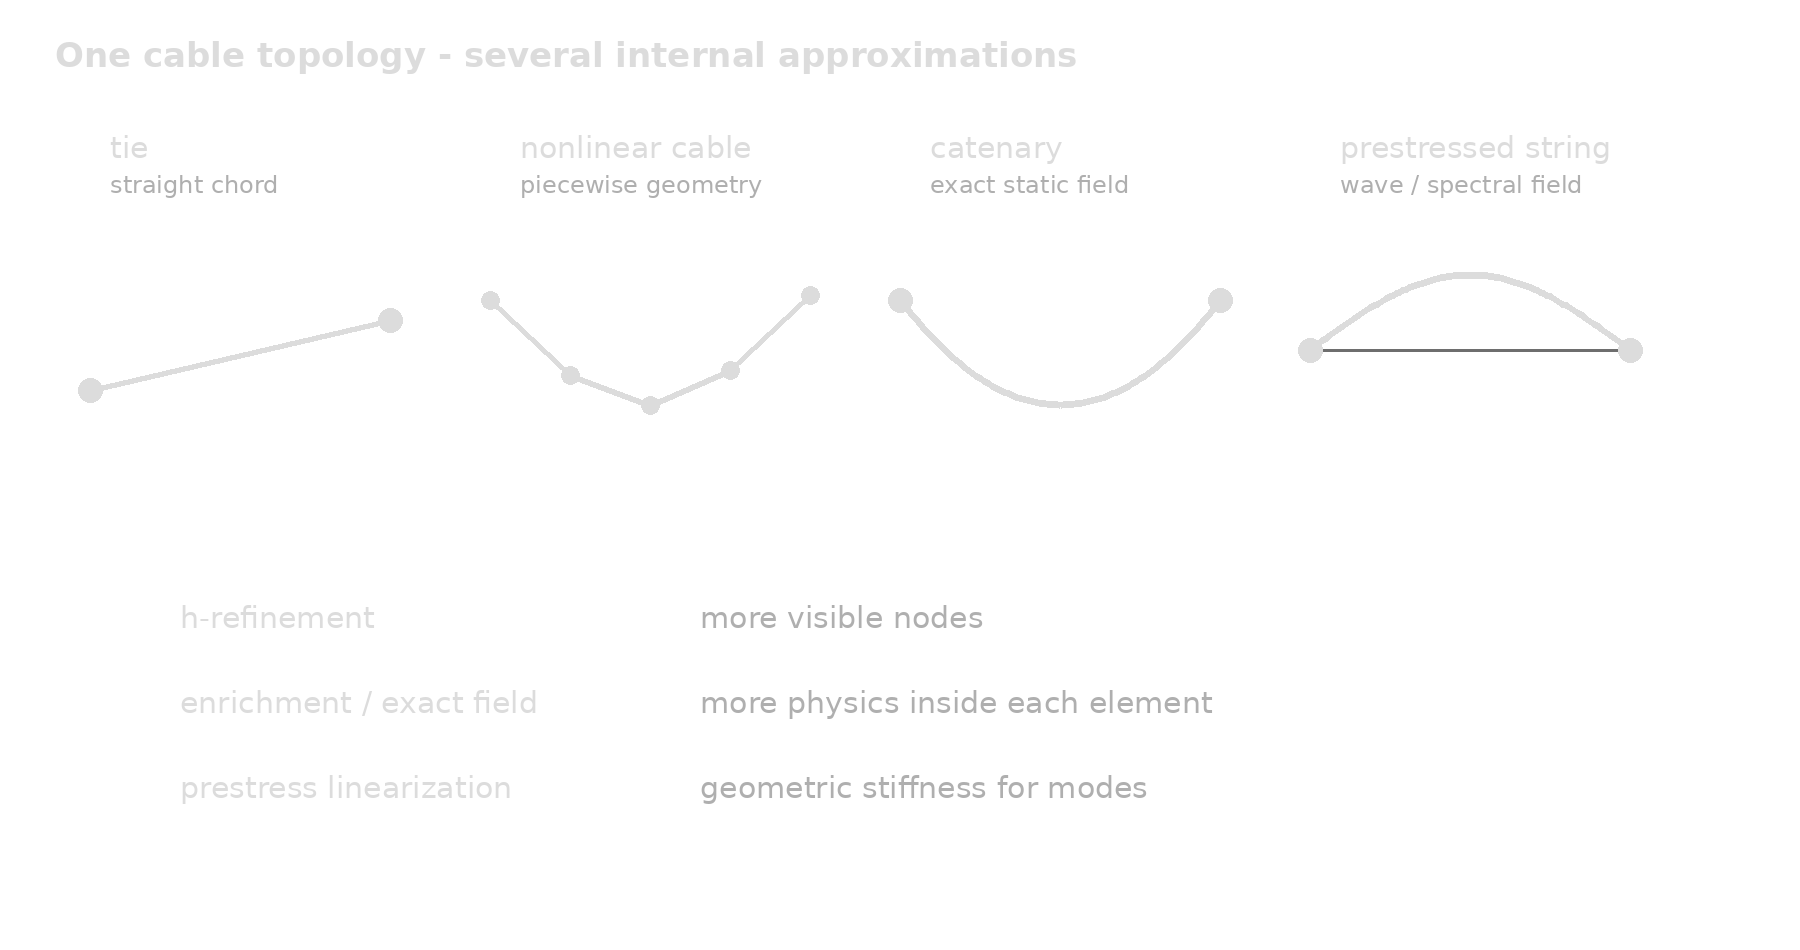
\includegraphics[width=0.88\textwidth]{img/fe_cable_formulations.png}
    \caption{The same end-node topology can support very different internal
    approximations: a straight tension-only tie, a piecewise nonlinear cable,
    an analytical catenary and a prestressed string/spectral representation.}
    \label{fig:fe-cable-formulations}
\end{figure}

\subsection{Level 1: Tension-Only Tie}

The simplest cable model is a two-node truss with no bending or shear
stiffness.  If $L_0$ is the reference length and $L$ the current chord length,

\begin{equation}
    \varepsilon=\frac{L-L_0}{L_0}.
\end{equation}

A tension-only constitutive law may be written

\begin{equation}
    N=\begin{cases}
        EA\varepsilon, & \varepsilon>0,\\
        0, & \varepsilon\le0.
    \end{cases}
\end{equation}

With geometric nonlinearity, a chain of these elements can sag and reorient.
However, one two-node straight tie cannot form a curved catenary inside the
element because it possesses no internal geometric coordinates.  Curvature is
created only by adding nodes.

This is pure $h$-refinement: improve the cable geometry by shortening the
piecewise straight segments.

\subsection{Level 2: Exact Catenary as the Internal Static Field}

A richer element can use the analytical equilibrium shape as its internal
approximation instead of a polynomial.  For a uniform, perfectly flexible,
inextensible cable hanging between equal-height supports with horizontal span
$L_x$, let $w$ be the weight per unit cable length and let

\begin{equation}
    a=\frac{H}{w},
\end{equation}

where $H$ is the constant horizontal tension component.  With the origin at
midspan, the catenary is

\begin{equation}\label{eq:catenary-shape}
    \boxed{
    y(x)=a\cosh\left(\frac{x}{a}\right)
    -a\cosh\left(\frac{L_x}{2a}\right)
    }.
\end{equation}

Its total cable length is

\begin{equation}\label{eq:catenary-length}
    \boxed{
    S=2a\sinh\left(\frac{L_x}{2a}\right)
    }.
\end{equation}

Thus the element can determine $a$ from the prescribed span and cable length,
then recover

\begin{equation}
    H=wa,
    \qquad
    V=\frac{wS}{2}
\end{equation}

at each support.  The complete static cable geometry exists inside the element
although only the two end nodes are visible globally.

A practical elastic catenary element generalizes this idea: endpoint force
parameters are chosen as local unknowns, the distributed-load equilibrium and
axial constitutive law are integrated along the cable, and a local nonlinear
iteration enforces the prescribed endpoint separation.  Differentiating the
endpoint residual gives the consistent element tangent.

\begin{python}
def symmetric_catenary(span, cable_length, weight_per_length, samples=11):
    if cable_length <= span:
        raise ValueError("a hanging catenary requires cable_length > span")

    # Solve S = 2 a sinh(span/(2a)) by bisection in a.
    a_lo = span * 1.0e-6
    a_hi = span

    def length_from_a(a):
        return 2.0 * a * math.sinh(span / (2.0*a))

    while length_from_a(a_hi) > cable_length:
        a_hi *= 2.0

    for _ in range(80):
        a_mid = 0.5 * (a_lo + a_hi)
        if length_from_a(a_mid) > cable_length:
            a_lo = a_mid
        else:
            a_hi = a_mid

    a = 0.5 * (a_lo + a_hi)
    H = weight_per_length * a
    V = 0.5 * weight_per_length * cable_length

    x = np.linspace(-0.5*span, 0.5*span, samples)
    y = np.zeros(samples, dtype=float)
    y_support = a * math.cosh(span / (2.0*a))
    for i, xi in enumerate(x):
        y[i] = a * math.cosh(xi/a) - y_support

    return x, y, H, V


x, y, H, V = symmetric_catenary(
    span=10.0,
    cable_length=10.5,
    weight_per_length=1.0,
)
print("midspan sag =", -y[len(y)//2])
print("horizontal tension H =", H)
print("vertical reaction V =", V)
\end{python}

\subsection{One Exact Element or Many?}

An exact local field does not imply that the whole cable must be one element.
A cable represented by 10 catenary elements is completely legitimate.  At an
internal node, global equilibrium enforces

\begin{equation}
    \m{f}^{(e)}_{R}+\m{f}^{(e+1)}_{L}+\m{f}_{\mathrm{ext}}=\m{0}.
\end{equation}

For a perfectly flexible cable there is no bending-moment continuity
requirement.  If there is no concentrated load at the shared node, force
equilibrium causes the adjacent element tangents to be compatible with the
continuous cable equilibrium.

For the special uniform catenary problem, one exact element may already
reproduce the assumed solution.  Subdivision becomes useful when

\begin{itemize}
    \item $EA$, mass or temperature varies along the cable,
    \item distributed loading changes between regions,
    \item intermediate attachments or concentrated loads are present,
    \item contact or pulleys change the load path,
    \item a local nonlinear solve is easier over shorter segments.
\end{itemize}

This is an important distinction between \emph{mesh refinement} and
\emph{approximation enrichment}.  A richer local element reduces the amount of
$h$-refinement required; it does not prohibit it.

\subsection{Level 3: Prestressed String and Geometric Stiffness}

Now consider small transverse vibration $w(x,t)$ about a straight equilibrium
state carrying constant tension $T$.  The governing equation is

\begin{equation}\label{eq:string-pde}
    \mu\ddot{w}-T w''=0,
\end{equation}

where $\mu=\rho A$ is mass per unit length.  The weak form contains

\begin{equation}
    \delta W_g
    =\int_0^L T\,\delta w' w'\,dx,
\end{equation}

so a two-node linear string segment has the prestress/geometric stiffness

\begin{equation}\label{eq:string-linear-km}
    \boxed{
    \m{K}_{g,e}=\frac{T}{L_e}
    \begin{bmatrix}1&-1\\-1&1\end{bmatrix},
    \qquad
    \m{M}_{e}=\frac{\mu L_e}{6}
    \begin{bmatrix}2&1\\1&2\end{bmatrix}
    }.
\end{equation}

The restoring stiffness is therefore created by the equilibrium tension, not by
beam bending stiffness.  For a fixed-fixed ideal string the exact frequencies
are

\begin{equation}\label{eq:string-exact-freq}
    \boxed{
    \omega_n=\frac{n\pi}{L}\sqrt{\frac{T}{\mu}},
    \qquad
    f_n=\frac{n}{2L}\sqrt{\frac{T}{\mu}}
    }.
\end{equation}

This is the simplest example of why a prestressed modal analysis must linearize
about the loaded equilibrium state: without $T$, the transverse string has no
restoring stiffness at all.

\subsection{Mesh Refinement versus a Physics-Informed Basis}

With ordinary linear elements, Equation~\eqref{eq:string-linear-km} is assembled
along the cable and the eigenfrequencies converge under mesh refinement.  The
following code avoids an eigensolver and instead evaluates the Rayleigh quotient
using the exact first-mode nodal pattern $q_i=\sin(\pi x_i/L)$:

\begin{python}
def assemble_linear_string(nelem, length, tension, mass_per_length):
    nnode = nelem + 1
    K = np.zeros((nnode, nnode), dtype=float)
    M = np.zeros((nnode, nnode), dtype=float)
    Le = length / nelem

    Ke = tension / Le * np.array([[1.0, -1.0], [-1.0, 1.0]])
    Me = mass_per_length * Le / 6.0 * np.array([[2.0, 1.0], [1.0, 2.0]])

    for e in range(nelem):
        ids = (e, e + 1)
        for a, I in enumerate(ids):
            for b, J in enumerate(ids):
                K[I, J] += Ke[a, b]
                M[I, J] += Me[a, b]
    return K, M


def first_string_rayleigh(nelem, length, tension, mass_per_length):
    K, M = assemble_linear_string(nelem, length, tension, mass_per_length)
    x = np.linspace(0.0, length, nelem + 1)
    q = np.sin(math.pi * x / length)
    omega2 = (q @ K @ q) / (q @ M @ q)
    return math.sqrt(omega2)


L = 10.0
T = 1000.0
mu = 2.0
omega_exact = math.pi / L * math.sqrt(T / mu)

for nelem in (2, 4, 10, 20):
    omega_h = first_string_rayleigh(nelem, L, T, mu)
    error = 100.0 * (omega_h / omega_exact - 1.0)
    print(nelem, omega_h, error)
\end{python}

For these values the first-mode Rayleigh estimate decreases from roughly 10.3\%
error with two elements to about 0.10\% with twenty elements.  This is ordinary
$h$-convergence.

But the continuum solution itself suggests another approximation space.  Choose
one global coordinate $a_1(t)$ and

\begin{equation}
    w^h(x,t)=a_1(t)\sin\left(\frac{\pi x}{L}\right).
\end{equation}

Then

\begin{equation}
    K_1
    =T\int_0^L\left(\frac{dN_1}{dx}\right)^2dx
    =\frac{T\pi^2}{2L},
\end{equation}

and

\begin{equation}
    M_1
    =\mu\int_0^L N_1^2\,dx
    =\frac{\mu L}{2}.
\end{equation}

Therefore

\begin{equation}
    \omega_1^2=\frac{K_1}{M_1}
    =\frac{\pi^2T}{\mu L^2},
\end{equation}

which gives Equation~\eqref{eq:string-exact-freq} \emph{exactly with one
coordinate}.  Adding

\begin{equation}
    N_n(x)=\sin\left(\frac{n\pi x}{L}\right)
\end{equation}

produces the corresponding exact ideal-string modes because the sine functions
are orthogonal in both the mass and geometric-stiffness integrals.

\begin{bbox}
\textbf{Global versus local trigonometric enrichment.}

A global sine basis knows the complete span and can reproduce selected ideal
string modes exactly, but its coordinates have global support.  A local bubble
such as $\sin(\pi x_e/L_e)$ can instead enrich every finite element while
preserving sparse assembly because it vanishes at the element ends.  The latter
is no longer globally exact, but it combines physics-informed enrichment with
ordinary FE locality.
\end{bbox}

\subsection{Level 4: Exact Dynamic Stiffness}

For harmonic motion $w(x,t)=W(x)e^{\mathrm{i}\omega t}$,
Equation~\eqref{eq:string-pde} becomes

\begin{equation}
    T W''+\mu\omega^2 W=0,
    \qquad
    k=\omega\sqrt{\frac{\mu}{T}}.
\end{equation}

The exact local field

\begin{equation}
    W(x)=A\cos(kx)+B\sin(kx)
\end{equation}

can be eliminated in favour of the endpoint values, giving the
frequency dependent dynamic stiffness

\begin{equation}\label{eq:string-dynamic-stiffness}
    \boxed{
    \m{K}_d(\omega)
    =\frac{Tk}{\sin(kL_e)}
    \begin{bmatrix}
        \cos(kL_e)&-1\\
        -1&\cos(kL_e)
    \end{bmatrix}
    }.
\end{equation}

A single local element therefore contains the exact wave solution rather than a
polynomial approximation.  Multiple such elements may still be assembled for
piecewise-varying $T$, $\mu$ or geometry.  The price is numerical: the global
free-vibration problem is no longer the ordinary polynomial eigenproblem
$\m{K}-\omega^2\m{M}$, but a nonlinear frequency equation

\begin{equation}
    \m{K}_d(\omega)\m{q}=\m{0}.
\end{equation}

Thus a richer approximation can reduce spatial DOFs while making the algebraic
solution procedure more sophisticated.

\subsection{Prestressed Modes of a Sagged Cable}

For a realistic sagged cable, first solve the nonlinear equilibrium

\begin{equation}
    \m{r}(\m{q}_0)=\m{0}
\end{equation}

for the reference geometry and tension distribution.  Then linearize the cable
about that state,

\begin{equation}
    \m{K}_{T}
    =\m{K}_{\mathrm{material}}
    +\m{K}_{\mathrm{geometric}}(\m{q}_0,N_0),
\end{equation}

and solve

\begin{equation}
    \boxed{
    (\m{K}_{T}-\omega^2\m{M})\M{\phi}=\m{0}
    }.
\end{equation}

The ideal string frequency is therefore a limiting case of the same prestressed
linearization used for general nonlinear structures.  With several cable
elements, each segment contributes the tangent associated with its own current
orientation and axial force.

\begin{notebooknote}[Element development lesson from the cable family]

The same two visible end nodes can support very different numerical models.
Choosing more elements ($h$-refinement), richer local polynomials or bubbles
($p$/enrichment), an exact static catenary, or an exact wave basis are different
ways of moving approximation error between geometry, interpolation and the
algebraic solution procedure.
\end{notebooknote}


\section[Cyclic-Symmetry Sector Formulation]{Design Example VI: Cyclic-Symmetry Sector Formulation}

A second route to a ``special element'' does not modify the continuum shape
functions at all. Instead, it changes the admissible discrete space.

Suppose a structure consists of $N$ identical sectors with sector angle

\begin{equation}
    \Delta\varphi=\frac{2\pi}{N}.
\end{equation}

Let corresponding nodes on the left and right sector boundaries be related by a
rotation $\m{R}_z(\Delta\varphi)$. For the static periodic case,

\begin{equation}
    \m{u}_R
    =\m{R}_z(\Delta\varphi)\m{u}_L.
\end{equation}

For harmonic index $m$, the cyclic/Bloch relation becomes

\begin{equation}\label{eq:cyclic-relation}
    \boxed{
    \m{u}_R
    =e^{\mathrm{i}m\Delta\varphi}
    \m{R}_z(\Delta\varphi)\m{u}_L
    }.
\end{equation}

The phase factor introduces complex coordinates for a general harmonic. The
rotation matrix is still required because displacement is a vector and the two
sector faces have different orientations in the global frame.

\begin{figure}[ht]
    \centering
    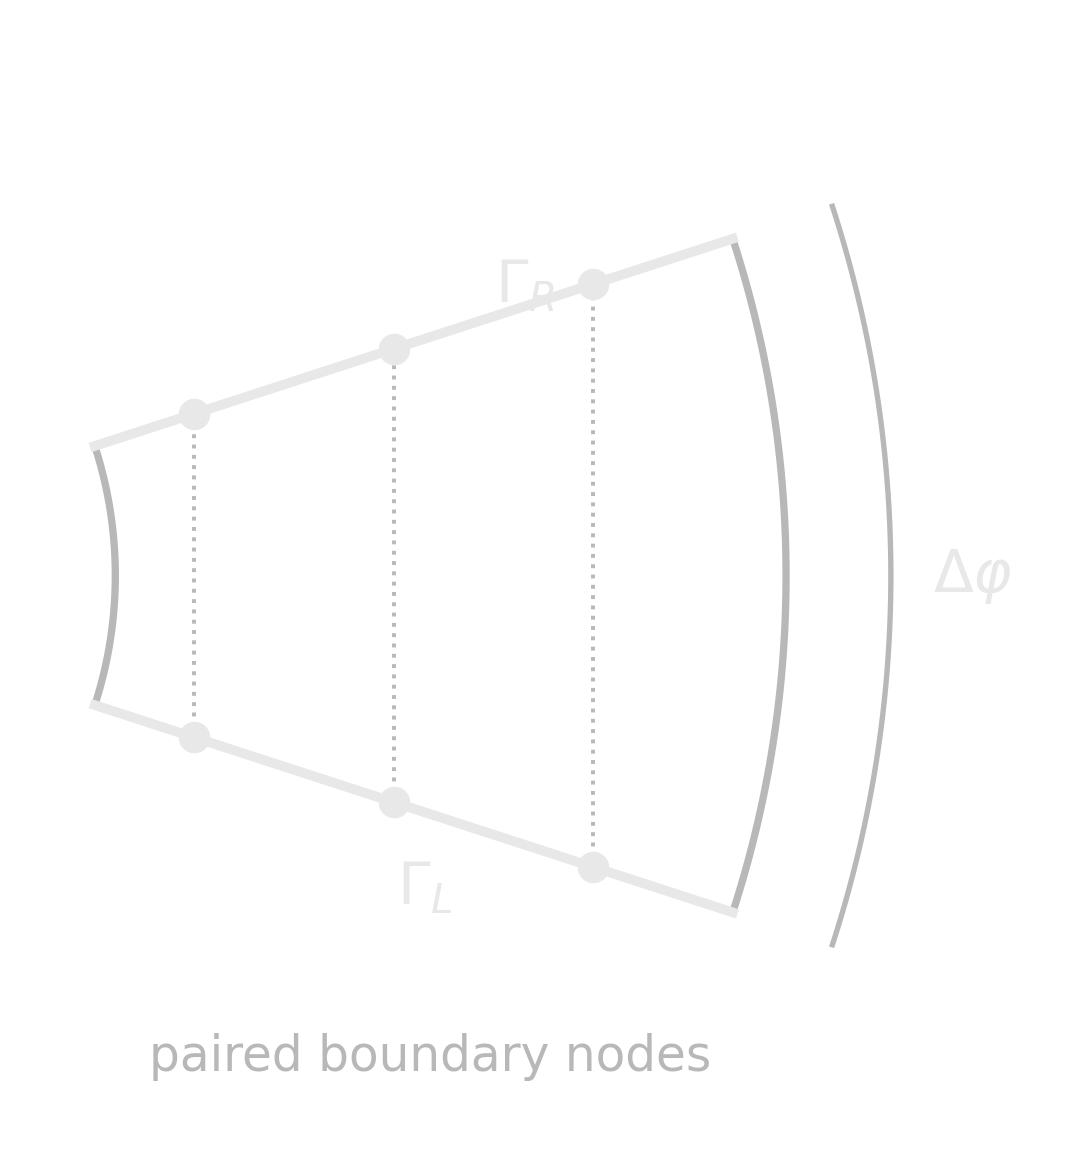
\includegraphics[width=0.63\textwidth]{img/fe_cyclic_sector.png}
    \caption{Cyclic symmetry can be imposed by restricting the admissible DOF
    space of an ordinary sector mesh. The continuum HEX8 interpolation need not
    change; corresponding boundary DOFs are related by a rotation and a harmonic
    phase.}
    \label{fig:fe-cyclic-sector}
\end{figure}

Collect all full sector DOFs as

\begin{equation}
    \m{q}_{\mathrm{full}}=\m{T}_m\m{q}_{\mathrm{red}},
\end{equation}

where $\m{T}_m$ inserts Equation~\eqref{eq:cyclic-relation} for every paired
boundary node. The reduced matrices follow from virtual work,

\begin{equation}\label{eq:cyclic-reduced-matrices}
    \boxed{
    \m{K}_m=\m{T}_m^H\m{K}\m{T}_m,
    \qquad
    \m{M}_m=\m{T}_m^H\m{M}\m{T}_m
    },
\end{equation}

where $(\cdot)^H$ denotes conjugate transpose.

This example is conceptually important because it shows that a new formulation
may arise in several ways:

\begin{itemize}
    \item changing the interpolation $\m{N}$,
    \item adding internal fields,
    \item changing numerical integration,
    \item changing the admissible discrete space through a transformation.
\end{itemize}

The last case connects directly to the multifreedom constraints of Chapter~3
and the reduction transformations used later in model reduction.

\subsection{A Minimal Cyclic Pair Builder}

The following function constructs the transformation for one pair of
three-translational-DOF boundary nodes. A full sector implementation repeats the
same block for every node pair and passes interior DOFs through unchanged.

\begin{python}
def rotation_z(angle):
    c = math.cos(angle)
    s = math.sin(angle)
    return np.array([
        [ c, -s, 0.0],
        [ s,  c, 0.0],
        [0.0, 0.0, 1.0],
    ], dtype=complex)


def cyclic_pair_transform(sector_angle, harmonic_index):
    phase = complex(
        math.cos(harmonic_index * sector_angle),
        math.sin(harmonic_index * sector_angle),
    )
    R = rotation_z(sector_angle)

    # q_full = [u_left, u_right], q_red = u_left.
    T = np.zeros((6, 3), dtype=complex)
    T[0:3, :] = np.eye(3, dtype=complex)
    T[3:6, :] = phase * R
    return T


def reduce_cyclic_matrix(Kfull, T):
    return T.conj().T @ Kfull @ T


angle = math.radians(30.0)
T2 = cyclic_pair_transform(angle, harmonic_index=2)
print(T2)
\end{python}

No eigensolver is needed to construct the cyclic matrix. The harmonic phase is
simply part of the transformation coefficients. An eigensolver only enters
later when the reduced harmonic stiffness and mass matrices are used to extract
sector modes.

\section{Verification of a New Element Formulation}

Deriving a matrix that compiles and produces numbers is not sufficient. Before a
new formulation is trusted, several independent tests should be performed.

\subsection{Rigid-Body Motion}

A displacement state representing pure rigid translation or rotation should
produce zero strain energy for an unconstrained linear elastic element,

\begin{equation}
    \m{q}_{rb}^T\m{K}_e\m{q}_{rb}=0.
\end{equation}

Unexpected resistance to a rigid-body mode usually indicates an incorrect
$\m{B}$ matrix, coordinate transformation or constraint in the element.

\subsection{Constant-Strain and Patch Tests}

If the exact continuum field has constant strain, the element should reproduce
it exactly when its approximation order claims to do so. A patch test goes
further by assembling several elements, often distorted, and checking that the
mesh reproduces the known polynomial state across interelement boundaries.

Passing a patch test is especially important for incompatible or enhanced
formulations because internal fields may violate pointwise displacement
compatibility while still satisfying the weaker consistency required for
convergence.

\subsection{Rank and Zero-Energy Modes}

The element stiffness should contain exactly the zero-energy modes expected from
its physics. A three-dimensional unconstrained solid has six rigid-body modes.
Additional zero-energy modes indicate an unstable interpolation or excessive
underintegration. Too few zero modes indicate artificial constraints or locking.

\subsection{Distortion Sensitivity}

An isoparametric element should be tested on skewed and distorted geometries.
The Jacobian determinant, gradient mapping and integration behaviour may be
excellent for a regular cube and poor for a warped brick. Element quality
metrics are therefore not cosmetic preprocessing data; they are indicators of
how far the numerical mapping has departed from the assumptions under which the
formulation performs well.

\subsection{Convergence}

A reliable element should converge toward the continuum solution under mesh
refinement. A single-element benchmark can expose gross errors, but it cannot
establish convergence. The final test of an element formulation is whether the
error decreases in a predictable manner as the approximation space is refined.

\section[Nonlinear Residual and Tangent]{Element Residual and Tangent: The Nonlinear View}

The closed-form linear stiffness matrix is a special case of the more general
residual formulation. For an element,

\begin{equation}
    \m{r}_e(\m{q}_e)
    =\m{f}_{\mathrm{ext},e}
    -\m{f}_{\mathrm{int},e}(\m{q}_e).
\end{equation}

A Newton iteration requires the tangent

\begin{equation}
    \m{K}_{T,e}
    =-\frac{\partial\m{r}_e}{\partial\m{q}_e}
    =\frac{\partial\m{f}_{\mathrm{int},e}}{\partial\m{q}_e}
      -\frac{\partial\m{f}_{\mathrm{ext},e}}{\partial\m{q}_e}.
\end{equation}

For linear elasticity with dead loads this reduces to the constant
Equation~\eqref{eq:element-stiffness}. For geometric or material nonlinearity,
however, the program must repeatedly update geometry, strains, stresses,
material state and tangent contributions at each integration point. The element
kernel therefore becomes a state-update algorithm rather than a one-time matrix
calculator.

This is the natural bridge to the nonlinear solution procedures developed later
in the book.

\section{Engineering View: What Is Actually Being Designed?}

A finite element is not simply its node count. ``Eight-node brick'' identifies a
topology, not a unique numerical formulation. Two elements with the same eight
corner nodes may differ in

\begin{itemize}
    \item interpolation, exposed nodal DOFs and internal modes,
    \item underlying continuum theory and the meaning assigned to any rotational coordinates,
    \item assumed strain fields,
    \item integration order,
    \item hourglass control,
    \item volumetric treatment,
    \item material integration,
    \item treatment of large rotations and deformation,
    \item mass matrix,
    \item internal condensation,
    \item stabilization parameters.
\end{itemize}

This is why commercial solvers may offer several ``HEX8'' or ``shell4'' options
with very different performance. The element name describes the visible mesh
topology; the formulation determines the numerical behaviour.

\begin{notebooknote}[A practical rule for deriving an element]

Start from the deformation states the element must reproduce, not from the
matrix you hope to obtain. Choose an approximation space that can represent
those states, derive its work-conjugate forces through virtual work or energy,
and only then decide how much of that approximation should remain as global
DOFs and how much can be integrated, condensed or stabilized locally.
\end{notebooknote}


\section{Summary}

The finite element method is a sequence of approximations rather than a single
matrix formula. Continuum equilibrium, kinematics and constitutive behaviour are
first written in a strong form, converted to a weak or variational statement,
and then approximated by a finite-dimensional interpolation.

For a linear displacement-based elastic element,

\begin{equation}
    \m{u}^h=\m{N}\m{q}_e,
    \qquad
    \M{\varepsilon}=\m{B}\m{q}_e,
\end{equation}

lead through either virtual work or deformation energy to

\begin{equation}
    \m{K}_e=\int\m{B}^T\m{D}\m{B}\,d\Omega,
    \qquad
    \m{M}_e=\int\rho\m{N}^T\m{N}\,d\Omega.
\end{equation}

In a program these integrals become loops over integration points, and global
assembly becomes loops over local-to-global DOF maps.

The Timoshenko example demonstrates that even a mathematically consistent
interpolation may lock if its discrete space cannot reproduce an important
limiting kinematic state. The enriched HEX8 example shows how internal
higher-order coordinates can improve the approximation while being condensed
before global assembly. The rotation-enriched brick shows how slope-like corner
coordinates can parameterize a richer quadratic Cauchy displacement field
without becoming independent material rotations. The cable family shows that
one topology can range from a simple tension-only tie to an exact catenary or a
spectral string depending on the chosen approximation space and tangent state.
The cyclic example shows yet another design mechanism: leave the ordinary
continuum element unchanged and transform the admissible DOF space itself.

These examples lead to a broader engineering conclusion: deriving an element
means designing a discrete approximation space, its energetically conjugate
forces, its numerical integration and its verification strategy. The Element
Atlas can then be read not as a collection of mysterious predefined matrices,
but as a catalogue of particular choices within this common framework.
